% Definições do documento
\documentclass[
	% -- opções da classe memoir --
	12pt,				% tamanho da fonte
	%openright,			% capítulos começam em pág ímpar (insere página vazia caso preciso)
	%twoside,			% para impressão em verso e anverso. Oposto a oneside
	oneside,	
	a4paper,			% tamanho do papel
	% -- opções da classe abntex2 --
	chapter=TITLE,		% títulos de capítulos convertidos em letras maiúsculas
	hyphens,            % Hífens nos links
	% -- opções do pacote babel --
	english,			% idioma adicional para hifenização
	french,				% idioma adicional para hifenização
	spanish,			% idioma adicional para hifenização
	brazil,				% o último idioma é o principal do documento
	]{abntex2}


% Configuração geral
% Pacotes
% Principais
\usepackage[T1]{fontenc}		% Selecao de codigos de fonte.
\usepackage[utf8]{inputenc}		% Codificacao do documento (conversão automática dos acentos)
\usepackage{indentfirst}		% Indenta o primeiro parágrafo de cada seção.
\usepackage{color}				% Controle das cores
\usepackage{graphicx}			% Inclusão de gráficos
\usepackage{subfigure}
\usepackage{microtype} 			% para melhorias de justificação
\usepackage{titlesec}           % para definir o formato do título
\usepackage{enumitem}           % Para realizar enumerações com ítens


% --------------
\usepackage{abntex2unifei}   % Adequações à Unifei. Usando localização relativa.
% --------------

% Citações
\usepackage[brazilian,hyperpageref]{backref}	 % Paginas com as citações na bibl
\usepackage[alf,abnt-emphasize=bf]{abntex2cite}  % Citações padrão ABNT, com referências em negrito



\usepackage{lipsum}				% para geração de dummy text




% Configurações de pacotes

% Configurações do pacote backref
% Usado sem a opção hyperpageref de backref
\renewcommand{\backrefpagesname}{Citado na(s) página(s):~}
% Texto padrão antes do número das páginas
\renewcommand{\backref}{}
% Define os textos da citação
\renewcommand*{\backrefalt}[4]{
	\ifcase #1 %
		Nenhuma citação no texto.%
	\or
		Citado na página #2.%
	\else
		Citado #1 vezes nas páginas #2.%
	\fi}%



% Configurações de aparência do PDF final

% alterando o aspecto da cor azul
\definecolor{blue}{RGB}{41,5,195}

% Espaçamentos entre parágrafo
% O tamanho do parágrafo é dado por:
\setlength{\parindent}{1.3cm}
% Controle do espaçamento entre um parágrafo e outro:
\setlength{\parskip}{0.3cm}  % tente também \onelineskip



%%%% CONFIGURAÇÕES DO TRABALHO %%%%
% Mude estes comandos para adequar seu trabalho a eles.

% Informações de dados para CAPA e FOLHA DE ROSTO
\titulo{Uma aplicação de aprendizado de máquina na classificação de galaxias}
\autor{Rafael J. Rangel}
\local{Itajubá}
\data{2020}
\instituicao{Universidade Federal de Itajubá - UNIFEI}
\tipotrabalho{Trabalho de Conclusão de Curso}
\orientador{Hektor Sthenos Alves Monteiro}
% O preambulo deve conter o tipo do trabalho, o objetivo, 
% o nome da instituição e a área de concentração.
%Estas informações serão impressas, por exemplo, na sua folha de rosto.
\preambulo{Trabalho de Conclusão de Curso apresentado à Universidade Federal de Itajubá como requisito para obtenção do grau de bacharel em Física.}


% Configurações gerais do PDF gerado (cor dos links, etc)
% Parte destes dados são gerados automaticamente.
\makeatletter
\hypersetup{
     	%pagebackref=true,
		pdftitle={\@title}, 
		pdfauthor={\@author},
    	pdfsubject={\imprimirpreambulo},
	    pdfcreator={trabalho},
		pdfkeywords={abntex2}{abntex2unifei}{latex}{texto}, 
		colorlinks=true,    % Links coloridos. Falso para criar caixas ao redor
        linkcolor=black,    % Cor de links internos (seções, etc)
    	citecolor=green,    % Cor de links para a bibliografia
    	filecolor=magenta,  % Cor de links para arquivos
		urlcolor=blue,      % Cor de links para URLs da web
		bookmarksdepth=4
}
\makeatother



% Compila o indice
\makeindex

\begin{document}

	% Elementos pré-textuais
	\pretextual
	% Os elementos a seguir aparecerão antes do início do artigo em si.

% Espaçamento de 1,5cm por linha
\OnehalfSpacing

% Capa
\imprimircapa

% Folha de rosto
\imprimirfolhaderosto

% Folha de aprovação
% COMANDO EXCLUSIVO DA ABNTEX2UNIFEI.
\imprimirfolhadeaprovacao{Trabalho de Conclusão de Curso apresentado à Universidade Federal de Itajubá como requisito para obtenção do grau de bacharel em Física.}


% Espaço reservado a dedicatórias
\begin{dedicatoria}
\null
\vfill
Dedico este trabalho aos meus colegas de curso, que assim como eu encerram uma difícil etapa da vida acadêmica.
\end{dedicatoria}


% Agradecimentos
\begin{agradecimentos}[Agradecimentos]
Agradeço imensamente aos meus professores em especifico ao meu orientador Hektor, sem o apoio do mesmo não conseguiria trilhar o caminho até aqui, agradeço aos meus colegas que compartilharam suas dificuldades e conquistas, por ultimo e mais importantes aos meus pais que mesmo sabendo das dificuldades do caminho que escolhi me apoiaram.
\end{agradecimentos}

% Epígrafe
\begin{epigrafe}
\null
\vfill \textit{“ Houve um tempo em que o homem enfrentou o universo sozinho e sem amigos. Agora ele tem criaturas para ajudá-lo; criaturas mais fortes que ele próprio, mais fiéis, mais úteis e totalmente devotadas a ele. A humanidade não está mais sozinha. ” }
\begin{flushright}
\textit{Isaac Asimov}
\end{flushright}
\end{epigrafe}



% Resumo
\begin{resumo}
Elemento obrigatório que apresenta uma sequência de frases objetivas e concisas, de 150 a 500 palavras, seguido de palavras-chave, as quais representam o conteúdo do trabalho. Geralmente apresenta: tema central, objetivo da pesquisa, aporte teórico, metodologia empregada, resultados e conclusões (tudo bem sucinto e sem citações).


Palavras-chave: Galaxias;Classificação;Visão Computacional;Aprendizado de Maquina.

\end{resumo}

\begin{resumo}[Abstract]
Apresentação, em inglês, do resumo que apresente o conteúdo de todo o trabalho (tema central, objetivo da pesquisa, aporte teórico, metodologia empregada, resultados e conclusões).


Keywords: 3 a 5 palavras-chave. Separadas entre si por ponto. Todas em inglês.
\end{resumo}


% Lista de Figuras
\pdfbookmark[0]{\listfigurename}{lof}
\listoffigures*
\cleardoublepage

% Lista de Tabelas
\pdfbookmark[0]{\listtablename}{lot}
\listoftables*
\cleardoublepage

% Lista de Abreviaturas e Siglas
\begin{siglas}
  \item[SDSS] Sloan Digital Sky Survey
  
  \item[RC3] Third Reference Catalogue of Bright Galaxies
  \item[VC] Visão Computacional
  \item[HOG] Histogram of Oriented Gradients 
  \item[HM] Hu Moments 
  \item[ML] Machine Learning
  \item[AM] Aprendizado de Máquina
  \item[TB] Tera Bytes
  \item[NB] Naive Bayes
  \item[LR] Logistic Regression
  \item[LDA] Linear Discriminant Analysis
  \item[K-NN] K-Nearest Neighbors 
  \item[SVM] Support Vector Machine 
  \item[DT] Decision Tree 
  \item[RF] Randon Forest 
  \item[MLP] Multilayer Perceptron 
  \item[GZ] Galaxy Zoo 
\end{siglas}

% Lista de Símbolos
\begin{simbolos}
  \item[$ \Gamma $] Letra grega Gama
  \item[$ \Lambda $] Lambda
  \item[$ \zeta $] Letra grega minúscula zeta
  \item[$ \in $] Pertence
  \item[O(n)] Ordem de um algoritmo
  \item[©] Copyright
\end{simbolos}

% Sumário
\pdfbookmark[0]{\contentsname}{toc}
\tableofcontents*
\cleardoublepage

	% Elementos textuais
	\textual
	
	% Inclui fontes não-citadas nas referências,
	% apenas para que apareçam como exemplo.
	
	% Introdução
	\chapter{Introdução} 

Na astrofísica moderna a abordagem de processos de otimização computacional é amplamente empregada, o presente trabalho visa a aplicação de ferramentas de otimização na classificação de galáxias, num contexto onde são utilizados métodos de aprendizado de máquina (AM).  

É importante conhecer o cenário onde a quantidade de informações a serem analisadas cresce diariamente do ponto de vista observacional astronômico, onde os métodos de análise mais indicado quando se trata desta quantidade massiva de dados é uma análise computacional. Praticamente toda analise de grande porte necessita de alguma técnica computacional. 

O nosso problema será a clássica análise de repositórios de imagens astronômicas. Onde desejamos classificar objetos extensos no céu, especificamente galáxias. Vamos empregar técnicas de AM, em conjunto com visão computacional, para tornar possível a uma classificação automática destes objetos quando apresentar um novo conjunto de dados desconhecidos. 

Na introdução abordaremos conceitos históricos sobre classificação de galáxias, métodos gerais de classificação com AM e uma introdução dos conceitos de visão computacional. 

\section{Galáxias} 

No século XVII vários astrônomos já haviam observado, entre as estrelas, a presença de corpos extensos e difusos, que foram chamados inicialmente de "nebulosas", sabemos que diferentes tipos de objetos estavam agrupados com esta terminologia, a maioria  deles pertencendo à nossa própria galáxia, dentre eles estavam nuvens de gás iluminadas por estrelas, cascas de gás ejetadas por estrelas em estágio final de evolução estelar, aglomerados de estrelas e outros objetos, mas algumas dessas nebulosas eram galáxias individuais, como a nossa Via Láctea. 

\begin{figure}[ht!] 
\centering 
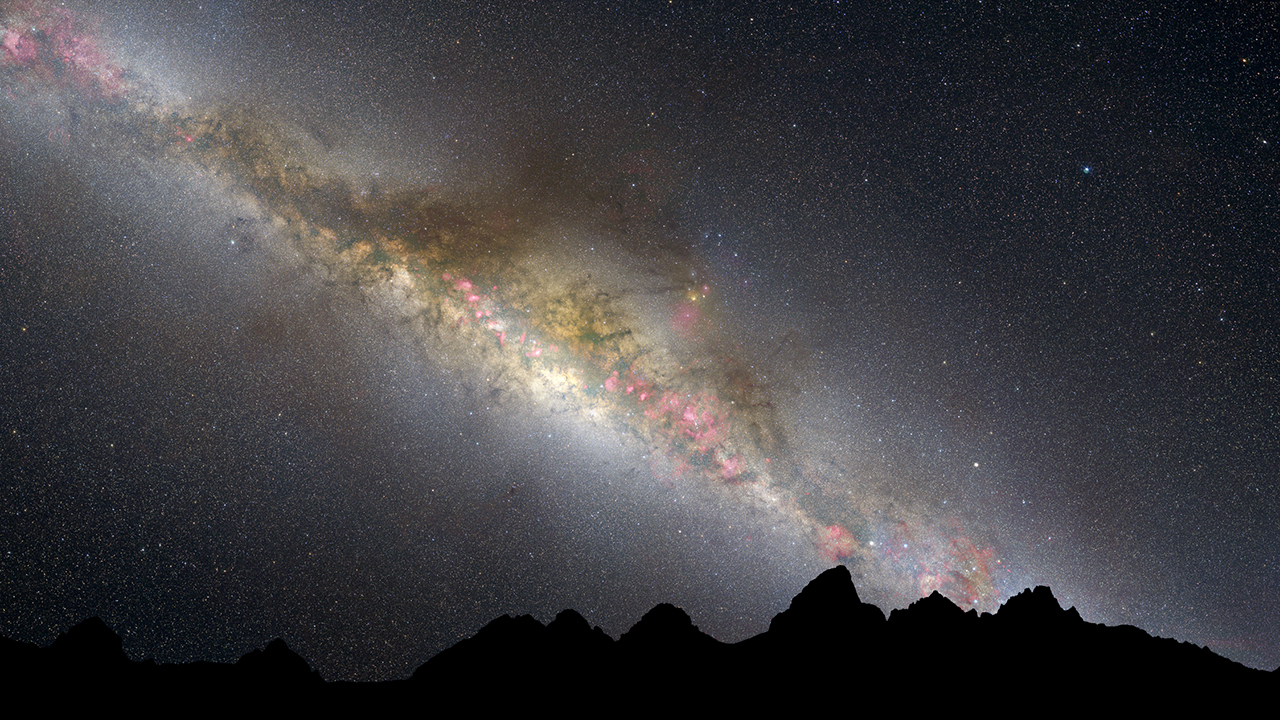
\includegraphics[width=15cm]{imagens/xlarge_web.jpg} 
\caption{Imagem da Via Láctea. Crédito: NASA, ESA e Z. Levay (STScI/AURA)} 
\label{fig:ViaLactea} 
\end{figure} 

O grande filósofo alemão Immanuel Kant (1724-1804), foi influenciado pelo astrônomo Thomas Wright (1711-1786) e propôs por volta de 1755, que algumas nebulosas poderiam ser sistemas estelares totalmente comparáveis à nossa galáxia. Kant comparou o sistema estelar em que vivemos com outros objetos observados similares e afirmou que apresentavam concordância com o conceito de que esses objetos elípticos são simplesmente universos ilhas, sendo assim outras "Vias Lácteas", a ideia ficou conhecia como a "hipótese dos universos-ilha", as especulações cosmológicas de Kant não foram bem aceitas, de forma que assunto permaneceu controverso na época. 

Até os anos 1900 cerca de 15000 nebulosas haviam sido catalogadas e descritas, sendo algumas identificadas corretamente como aglomerados estelares, e outras como nebulosas gasosas, o maior problema se tratava da distância que não era conhecida, assim não era possível saber se objeto estava contido na nossa galáxia ou fora dela, isso era o que impossibilitava explicar a maior parte dos objetos. 

Alguns dos maiores protagonistas nessa controvérsia foram Harlow Shapley (1885-1972), do observatório Mount Wilson Observatory, e Heber Doust Curtis (1872-1942), do observatório Lick Observatory. Shapley defendia que as nebulosas espirais eram objetos da nossa Galáxia, e Curtis defendia a ideia oposta, de que eram objetos extragalácticos, essa discussão culminou num famoso debate em abril de 1920, frente à Academia Nacional de Ciências. 

O debate terminou inconclusivo devido à dificuldade de se medir as grandes distâncias em Astronomia, mas no final de 1923, o mistério foi resolvido por Edwin Powell Hubble (1889-1953), que estimou a distância até a nebulosa de Andrômeda (M31), demonstrando que a mesma estava fora da Via Láctea. Utilizando a calibração das estrelas variáveis Cefeídas, ideia proposta por Henrietta Leavitt e sugerida para medir distâncias até as nebulosas por Harlow Shapley, Hubble fundou uma nova área do conhecimento, que foi chamada Astronomia Extragaláctica. 

\begin{figure}[ht!] 
\centering 
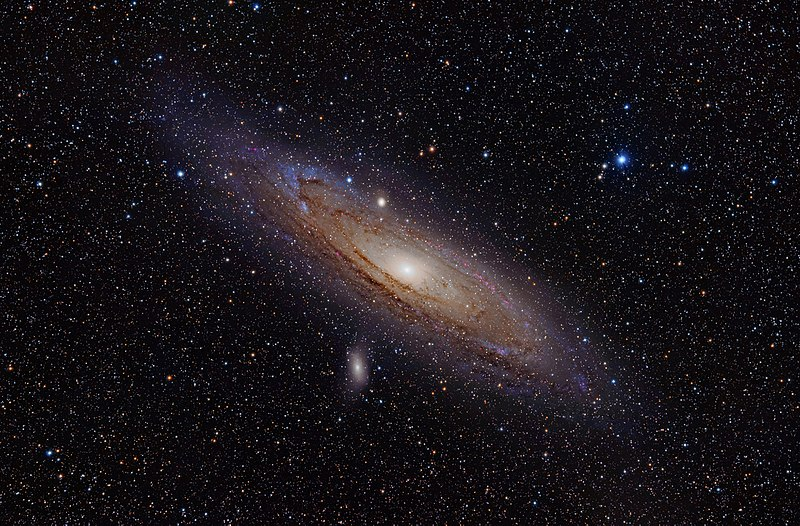
\includegraphics[width=14cm]{imagens/800px-Andromeda_Galaxy_(with_h-alpha).jpg} 
\caption{A galáxia de Andrômeda é uma galáxia espiral a aproximadamente 2,5 milhões de anos-luz de distância na constelação de Andrômeda. A imagem também mostra Messier 32 e 110, bem como o NGC 206 (uma nuvem de estrelas brilhantes na galáxia de Andrômeda) e a estrela Nu Andrômeda. Crédito: Adam Evans.} 
\label{fig:Andrômeda} 
\end{figure} 

A cosmologia observacional dava seus primeiros passos, por volta de 1920-1930, utilizando medidas de velocidade e distância, para uma amostra de vinte e duas nebulosas (galáxias), Hubble descobriu a expansão do Universo. 

\subsection{Classificação de Galáxias e Sequência de Hubble} 

Em geral galáxias diferem bastante entre si, mas na maioria delas observamos uma regularidade, quando observadas em projeção contra o céu, se enquadram em duas classes básicas: espirais e elípticas.  

Galáxias que não apresentam forma definida são chamadas de irregulares \cite{extragalatic}. Sabemos que as galáxias nascem nas regiões de maior condensação da matéria escura, assim existe uma certa distribuição destas condensações que é aleatória.  

Ressaltamos dois aspectos na formação das galáxias a simetria e a assimetria, no caso de uma distribuição simétrica, não haverá momentum angular líquido, e temos a formação de uma galáxia elíptica, na distribuição assimétrica as condensações em uma região do espaço produzem força de maré que gera momentum angular na nuvem, o que forma uma galáxia espiral. 

O esquema mais utilizado para classificação é a sequência de Hubble \cite{bergh1998galaxy}. Quando o esquema foi concebido pensava-se que o mesmo poderia fornecer informações sobre a evolução das galáxias \cite{1926CMWCI.324....1H}. 

\begin{figure}[ht!] 
\centering 
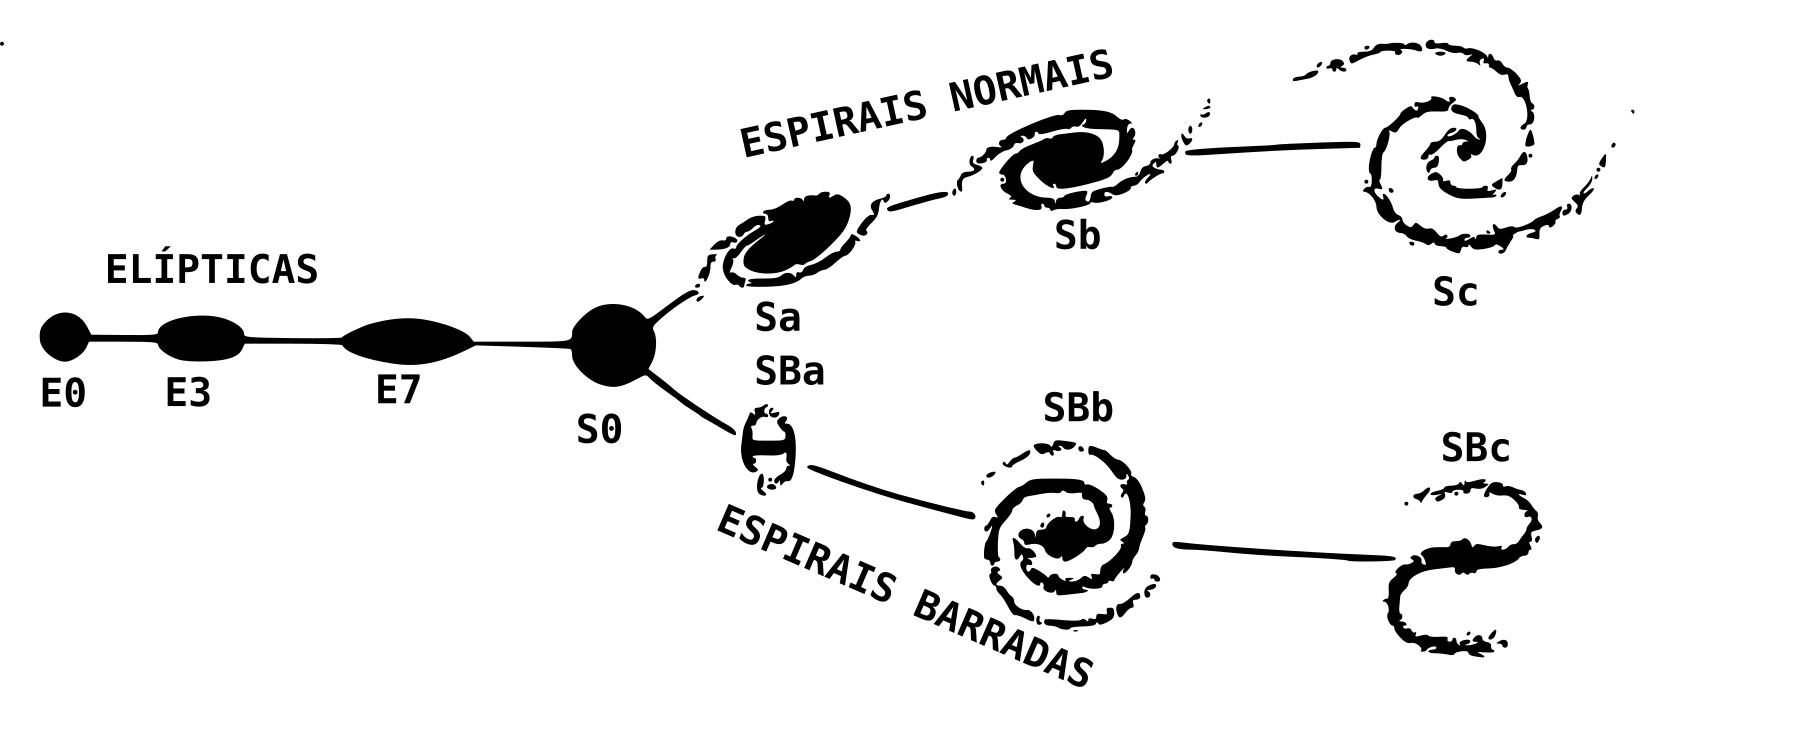
\includegraphics[width=15cm]{imagens/The-Hubble-tuning-fork-diagram.png} 
\caption{Tipos de galáxia de acordo com o esquema de classificação de Hubble. A letra E representa galáxia elíptica, a letra S uma galáxia espiral e as letras SB representam uma galáxia espiral barrada. Crédito: Wikipédia/Domínio Público.} 
\label{fig:ClassificaçãodeHubble} 
\end{figure} 

\subsection{Galáxias Elípticas} 

As galáxias elípticas são um tipo de galáxia, que apresenta uma forma aproximada a uma elipsoide \cite{extragalatic}. Estão distribuídas mais igualmente entre as três dimensões do espaço. As estrelas possuem órbitas aleatórias o que se assemelha com as órbitas planares. A maioria apresenta pouco gás, pouca poeira e poucas estrelas jovens, as galáxias elípticas parecem muito com o núcleo e halo das galáxias espirais. 

A divisão Hubble das galáxias elípticas levou em conta o achatamento do núcleo. As classes vão de E0 a E7 de acordo com o seu grau de achatamento. As galáxias E0 apresentam forma circular vistas de frente. Conforme achatamos esse círculo de modo gradativo para uma elipse representamos a sequência de E0 a E7 \cite{bergh1998galaxy}. Essa classificação leva em conta a aparência da galáxia, não na sua verdadeira forma. Uma galáxia E0 pode ser elíptica realmente esférica tanto quanto pode ser uma elíptica mais achatada vista de frente, já uma E7 tem que ser uma elíptica achatada vista de perfil, mas nenhuma elíptica vai parecer tão achatada quanto uma espiral vista de perfil. 
\begin{figure}[ht!] 
\centering 
\subfigure[ref1][M89 (NGC 4552))]{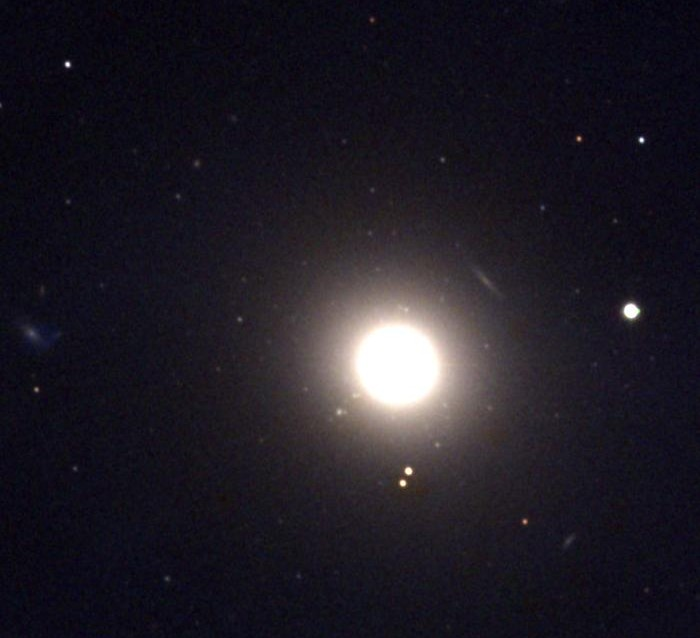
\includegraphics[width=5cm]{imagens/m89.jpg}}
\qquad 
\subfigure[ref2][M110 (NGC 205)]{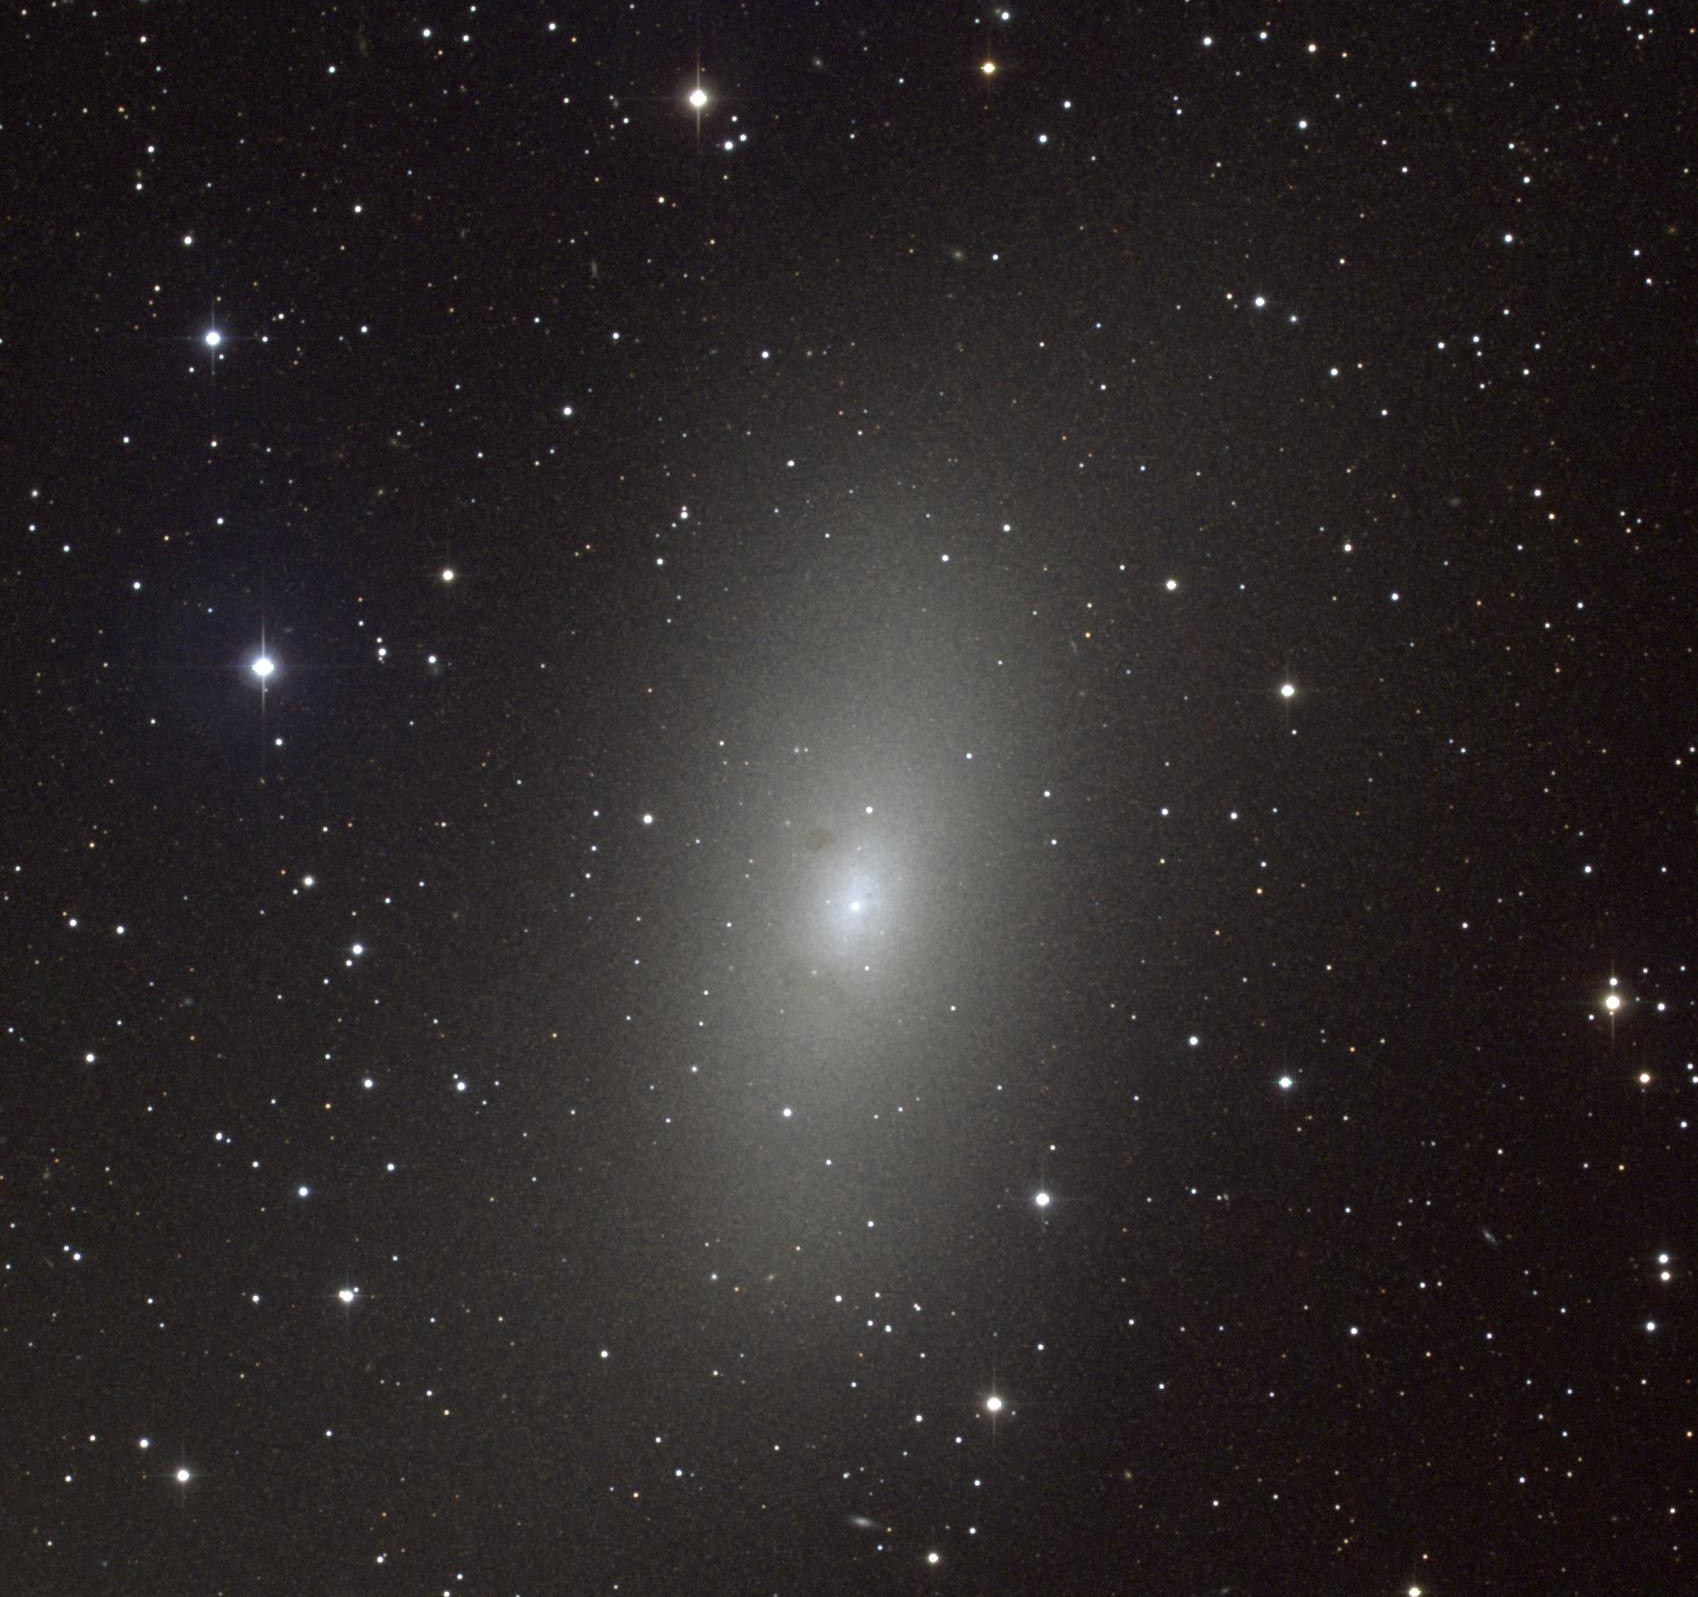
\includegraphics[width=5cm]{imagens/m110.jpg}} 
\caption{(a) M89 (NGC 4552). Galáxia elíptica do tipo E0, a 60 milhões de anos-luz da Terra, na constelação de Virgem. Magnitude aparente de 9.8. Pertencente ao enxame de galáxias de Virgem, foi descoberto por Charles Messier em 1781. Crédito: NOAO/AURA/NSF. \newline  (b) M110 (NGC 205) Galáxia elíptica do tipo E6, a 2.9 milhões de anos-luz da Terra, na constelação de Andrómeda. Magnitude aparente de 8.5. É a segunda companheira de M31, em conjunto com M32. Foi descoberto em 1773 por Charles Messier. Crédito: NOAO/AURA/NSF.} 
\label{fig:galáxiasElipticas} 
\end{figure} 

As galáxias elípticas são quase um terço de todas as galáxias \cite{extragalatic}. Têm dimensões variadas que vão desde galáxias anãs, até galáxias gigantes. As maiores podem ter até 10 trilhões de massas solares e cerca de milhões anos-luz de diâmetro. Sendo as mais comuns galáxias elípticas anãs que contêm poucos milhões de massas solares e apenas cerca de alguns mil anos-luz de diâmetro. A Galáxia de Andrômeda (M31), tem duas companheiras que são galáxias elípticas anãs. 

\begin{figure}[ht!]
\centering 
\subfigure[ref1][M87 (NGC 4486)]{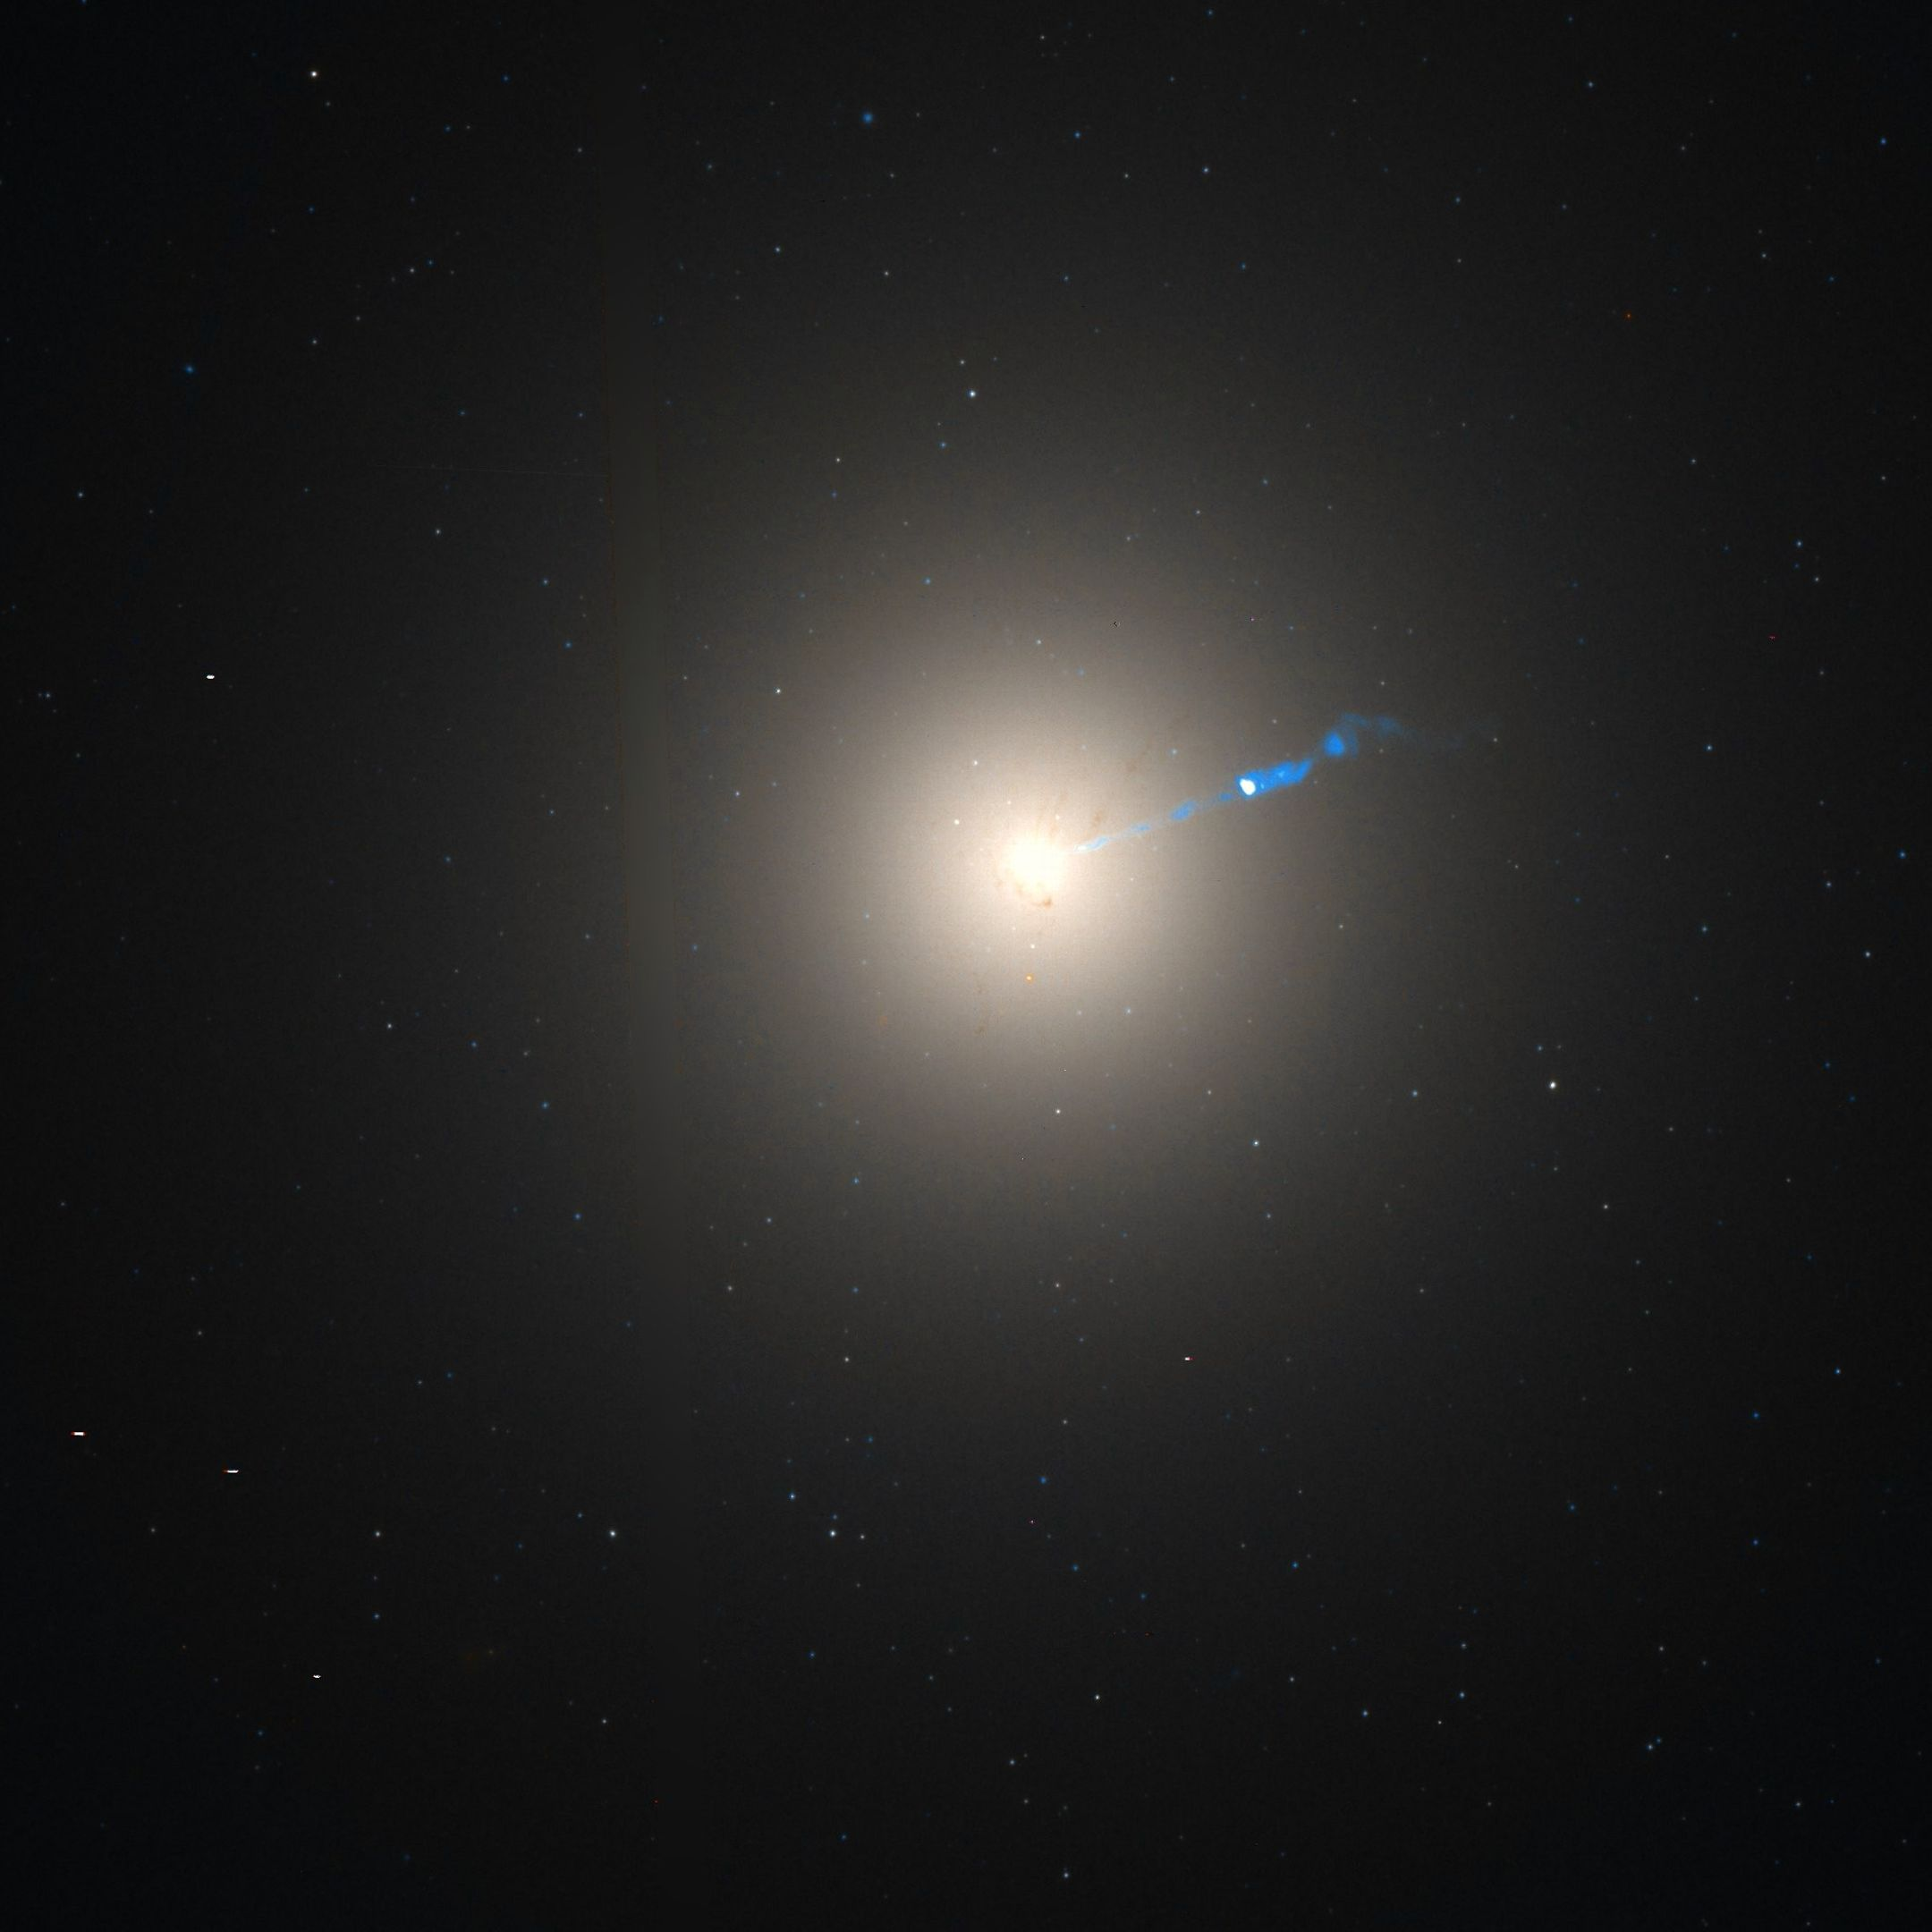
\includegraphics[width=5cm]{imagens/m87.jpg}} 
\qquad 
\subfigure[ref2][M60 (NGC 4649)]{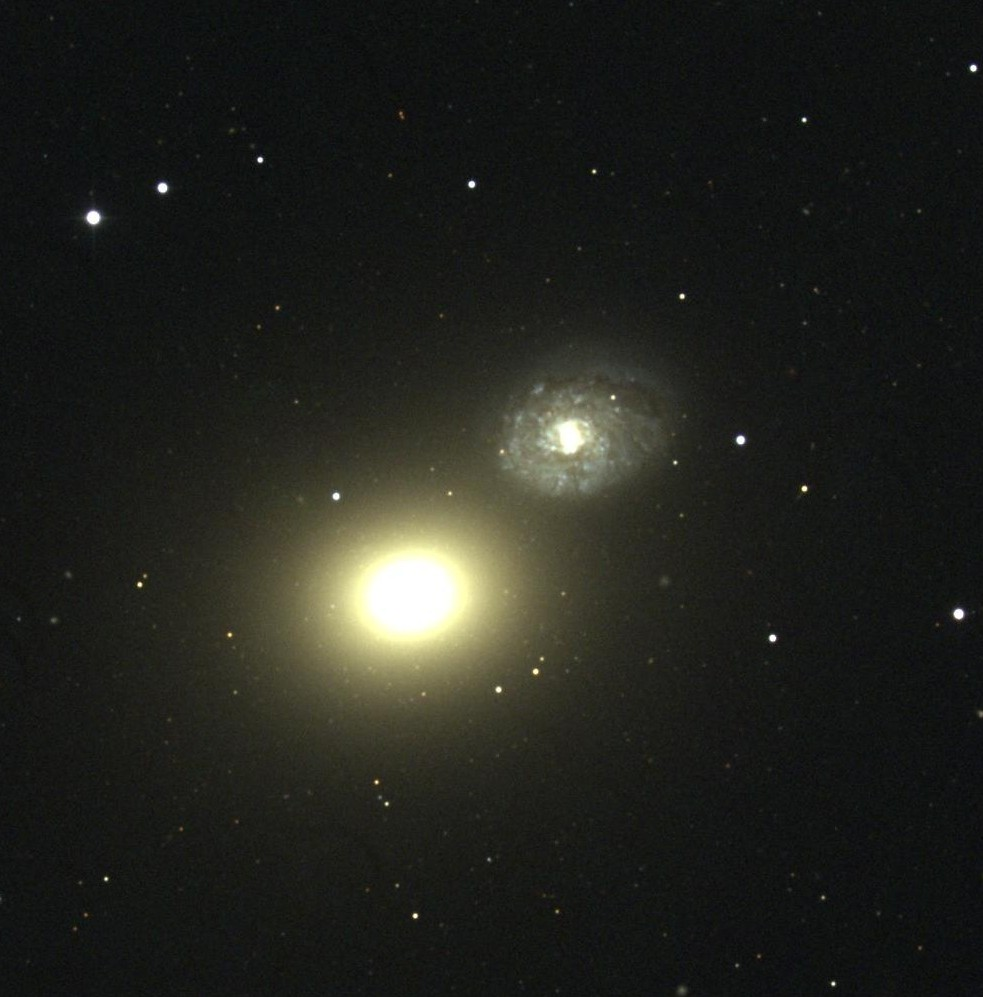
\includegraphics[width=5cm]{imagens/m60.jpg}} 
\caption{(a) M87 também chamada de Virgo A ou NGC 4486 é uma galáxia elíptica supergigante localizada na constelação de Virgem, uma das mais massivas do Universo local. Ela possui uma grande população de aglomerados globulares e um distinto jato de plasma energético que se origina em seu núcleo e estende-se por pelo menos 4,9 mil anos-luz, viajando em uma velocidade relativista. Magnitude aparente 7.19. Messier 87 também é um dos pontos de rádio mais brilhantes no céu e um alvo popular para astrônomos. Crédito: Hubble. \newline  (b) M60 (NGC 4649). Galáxia elíptica do tipo E2, com aproximadamente 120.000 anos-luz de diâmetro, encontra-se na constelação de Virgo sendo o terceiro objeto mais brilhante do aglomerado de Virgem. Crédito: HUBBLE.} 
\label{fig:galáxiasElipticas2} 
\end{figure} 

\subsection{Galáxias Espirais} 

As galáxias espirais são galáxias que quando vistas de frente, apresentam uma clara estrutura espiral. Possuem um núcleo em forma de disco e braços espirais, elas apresentam diferenças entre si principalmente quanto ao tamanho do núcleo e ao grau de desenvolvimento dos braços espirais\cite{extragalatic}.  

A formação estelar e composta por estrelas jovens e velhas, sugerindo que não se formaram a partir de outra galáxia mais antiga. O núcleo é formado predominantemente por estrelas mais velhas e seus braços apresentam uma maior atividade de formação estelar. Os núcleos das galáxias espirais têm uma tonalidade mais laranja e os braços uma tonalidade mais azul, fatores importantes para classificação. 

As galáxias espirais tem diâmetros que variam de 20 mil até mais de 100 mil anos-luz e suas massas variam de 10 bilhões até 10 trilhões de vezes a massa do Sol. Nossa Via-Láctea, é uma galáxia espiral grande e massiva. 

São divididas nas categorias S não barradas e SB barradas. As S também se subdividem nas categorias Sa, Sb, e Sc, levando em conta o grau de desenvolvimento, enrolamento dos braços espirais, tamanho do núcleo comparado com relação ao disco. 

As galáxias do tipo Sa têm núcleo maior, braços pequenos e bem enrolados, as Sb tem núcleo e braços intermediários, as Sc tem núcleo menor, braços grandes e mais abertos.  

\begin{figure}[ht!] 
\centering 
\subfigure[ref1][M96 (NGC 3368)]{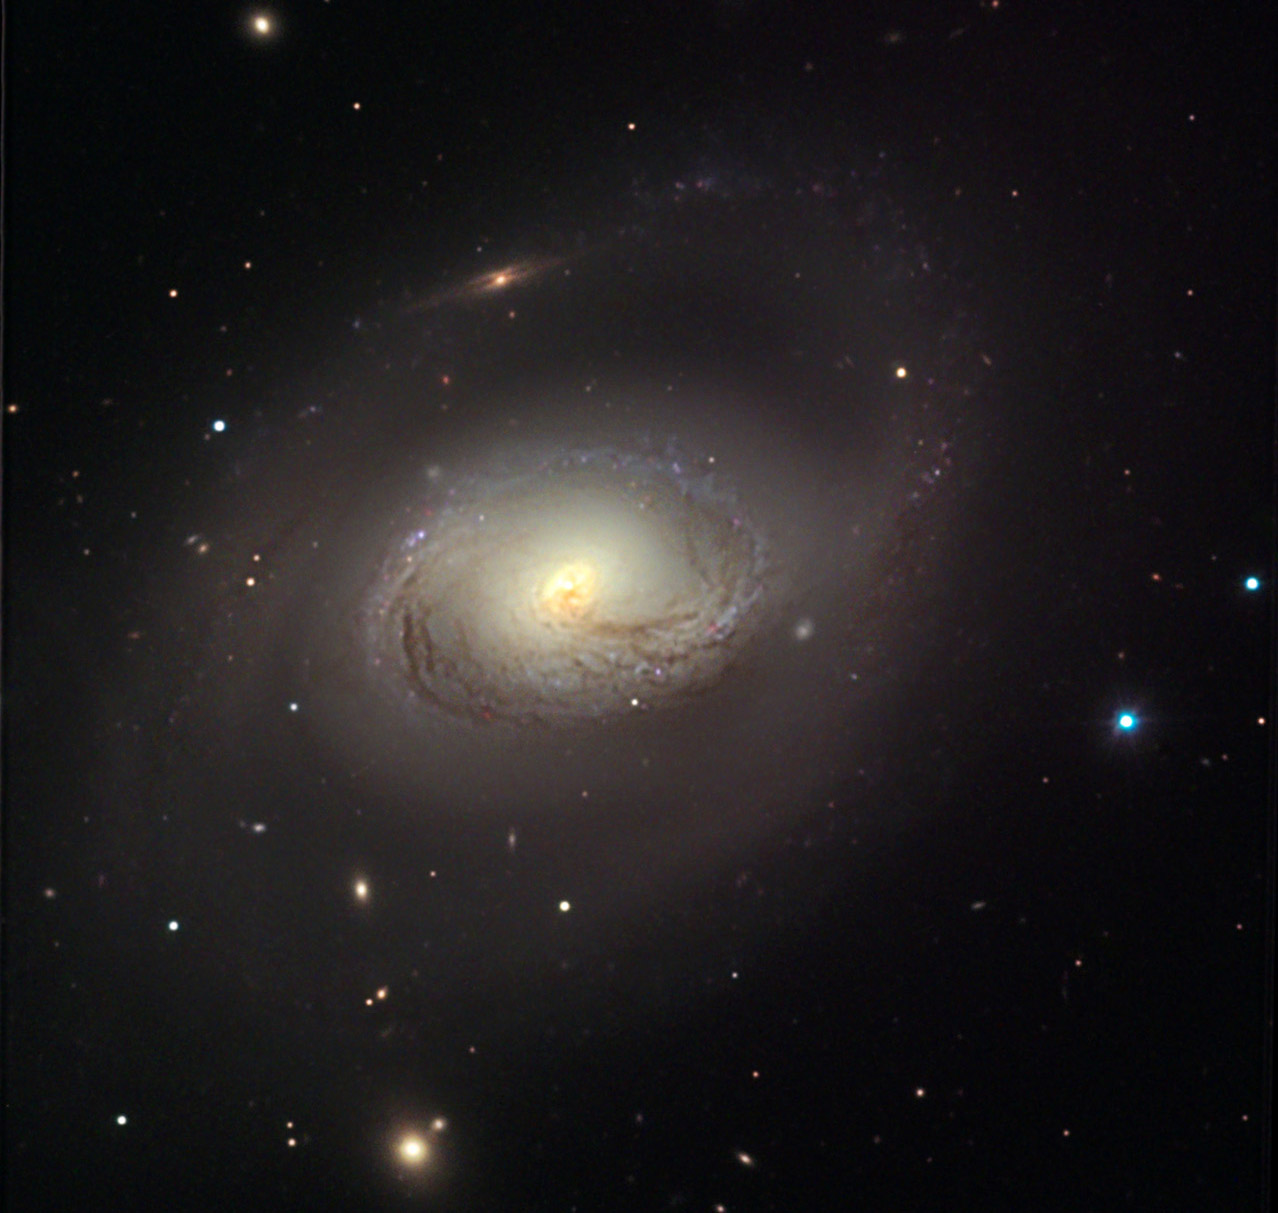
\includegraphics[width=4cm]{imagens/m96.jpg}} 
\qquad 
\subfigure[ref2][M63 (NGC 5055)]{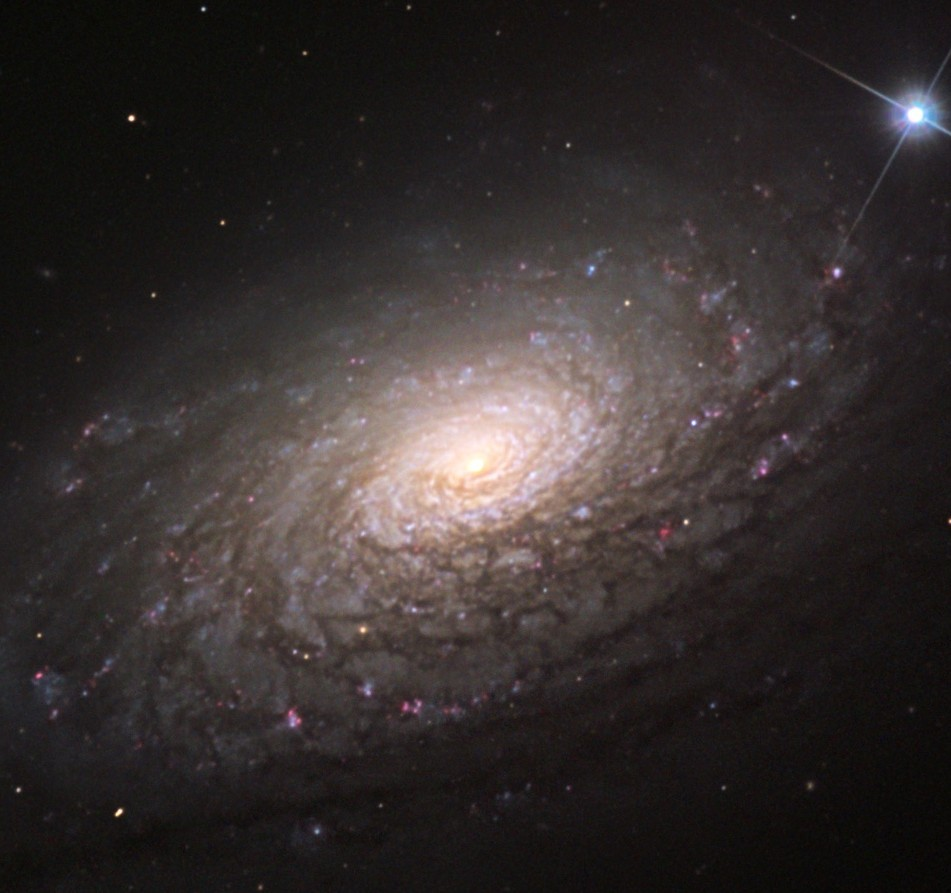
\includegraphics[width=4cm]{imagens/m63.jpg}} 
\qquad 
\subfigure[ref2][M64 (NGC 628)]{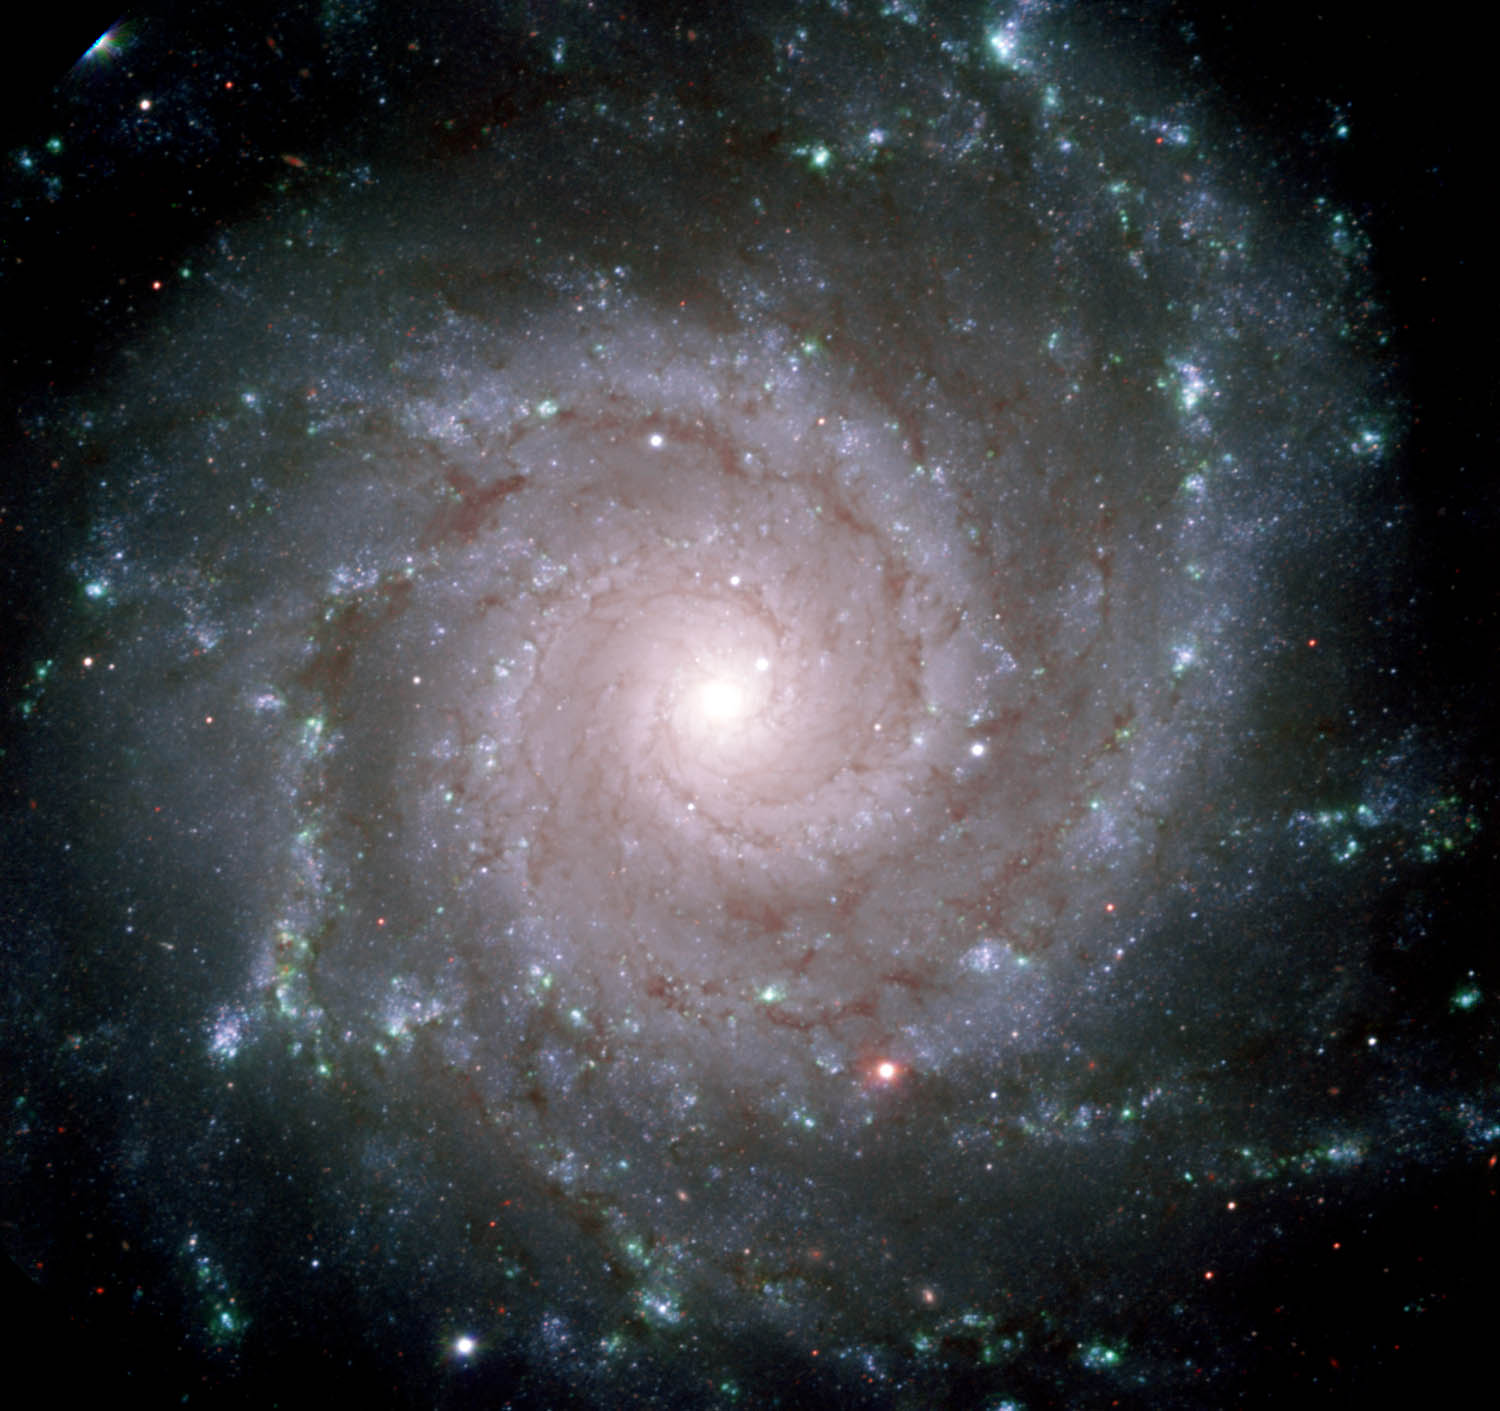
\includegraphics[width=4cm]{imagens/m74.jpg}} 
\caption{(a) M96 (NGC 3368). Galáxia espiral do tipo Sa, a 38 milhões de anos-luz da Terra, na constelação de Leão. Magnitude de 9.2. É o membro mais brilhante do grupo de galáxias M96, também conhecido por grupo Leo I. Crédito: Adam Block /NOAO/AURA/NSF,\newline (b) M63 (Galáxia do Girassol ou NGC 5055). Galáxia espiral do tipo Sb, a 37 milhões de anos-luz da Terra, na constelação de Cães de Caça. Magnitude aparente de 8.6. Ao que parece forma um grupo físico com a galáxia do Cata-vento e outras mais pequenas: o grupo M51. Crédito: Bruce Hugo e Leslie Paul/Adam Block/NOAO/AURA/NSF,\newline (c) M64 (NGC 628). Galáxia espiral do tipo Sc, a 35 milhões de anos-luz da Terra, na constelação de Peixes. Magnitude de 9.4. Aclamada por muitos como a "galáxia espiral perfeita". Crédito: Observatório Gemini, Equipa GMOS} 
\label{fig:galáxiasElipticas3} 
\end{figure} 

Algumas galáxias que têm núcleo, disco e halo, mas não têm traços de estrutura espiral, são classificadas como S0 na sequência Hubble, chamadas de lenticulares, na maior parte galáxias relativamente isoladas no universo que não tiveram interações gravitacionais próximas por um período muito longo de tempo. São dificilmente distinguíveis das galáxias elípticas devido à sua aparência e classificadas incorretamente no passado. As galáxias espirais e lenticulares juntas são chamadas de galáxias discoidais. 

\begin{figure}[ht!] 
\centering 
\subfigure[ref1][M61 (NGC 4303)]{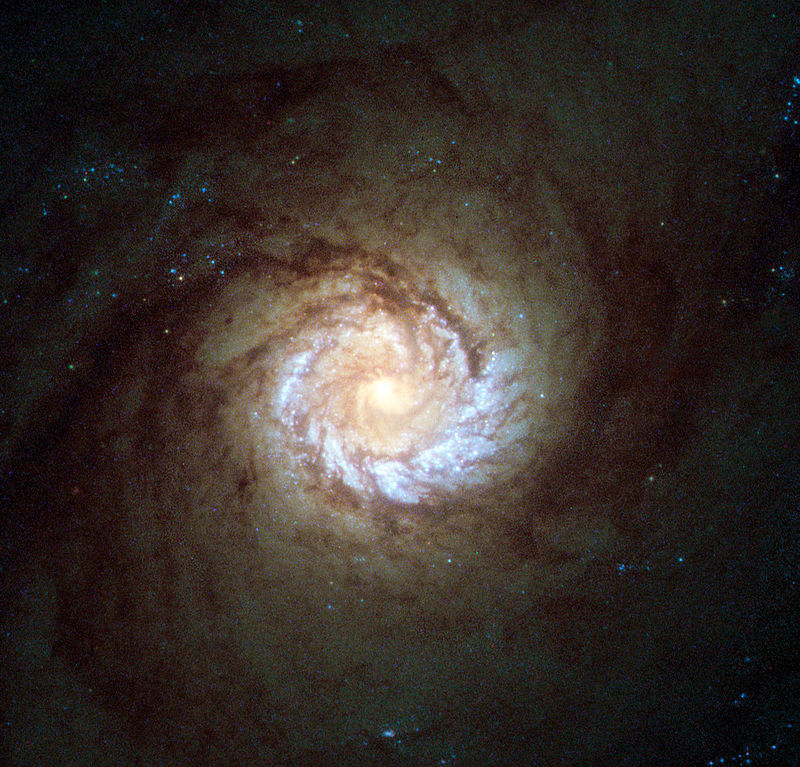
\includegraphics[width=5cm]{imagens/m61.jpg}} 
\qquad 
\subfigure[ref2][M102 (NGC 5866)]{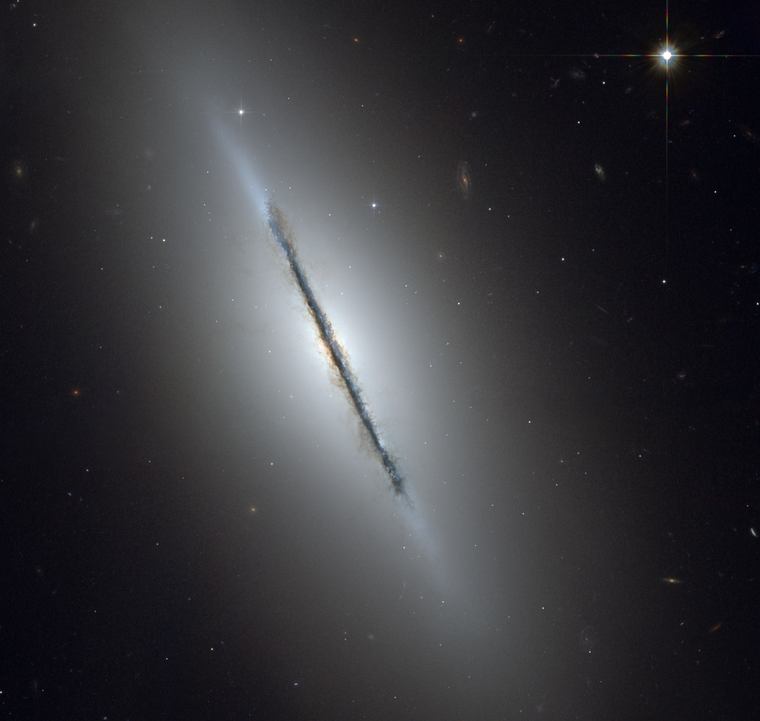
\includegraphics[width=5cm]{imagens/NGC5866.png}} 
\caption{(a)M61 (NGC 4303). Galáxia do tipo S0, chamada de Messier 61 , pertencem a um grupo de galáxias conhecido como Superaglomerado Virgo na constelação de Virgem (A Virgem) - um grupo de aglomerados de galáxias que contêm até 2000 galáxias espirais e elípticas no total. O Messier 61 é um tipo de galáxia conhecida como galáxia de explosão estelar. Magnitude de 10.18 . Crédito: ESA / Hubble e NASA. Agradecimento: Det58.\newline (b) M102 (NGC 5866). Galáxia do tipo S0. É uma galáxia lenticular localizada a cerca de quarenta milhões de anos-luz (aproximadamente 12.26 megaparsecs) de distância na direção da constelação do Dragão. Magnitude aparente de 9.9. Existe a possibilidade de Messier 102 ser uma duplicata de Messier 101. Crédito: NASA, ESA, e The Hubble Heritage Team (STScI/AURA)} 
\label{fig:galáxiasElipticas4} 
\end{figure} 

Existem ainda outras classificações que se ramificam da sequência de Hubble \cite{bergh1998galaxy}, o sistema de Vaucouleurs \cite{1959HDP....53..275D} é um bom exemplo. Dentro deste sistema as galáxias lenticulares também são classificadas como não barradas (SA0) ou barradas (SB0), com a notação S0 reservada para as galáxias para as quais é impossível saber se uma barra está presente ou não.  

É importante observar que mais da metade das galáxias discoidais apresentam uma barra atravessando o núcleo e são chamadas barradas, na classificação de Hubble identificadas pelas iniciais SB. As barradas também se subdividem nas categorias SB0, SBa, SBb, e SBc.  

\begin{figure}[ht!] 
\centering 
\subfigure[ref1][NGC 1433]{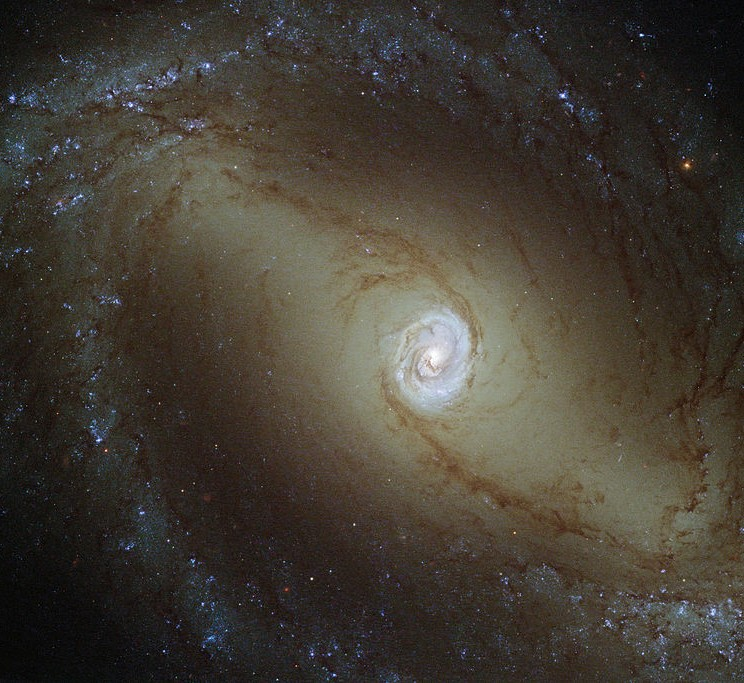
\includegraphics[width=4cm]{imagens/ngc1433.jpg}} 
\qquad 
\subfigure[ref2][NGC 1365]{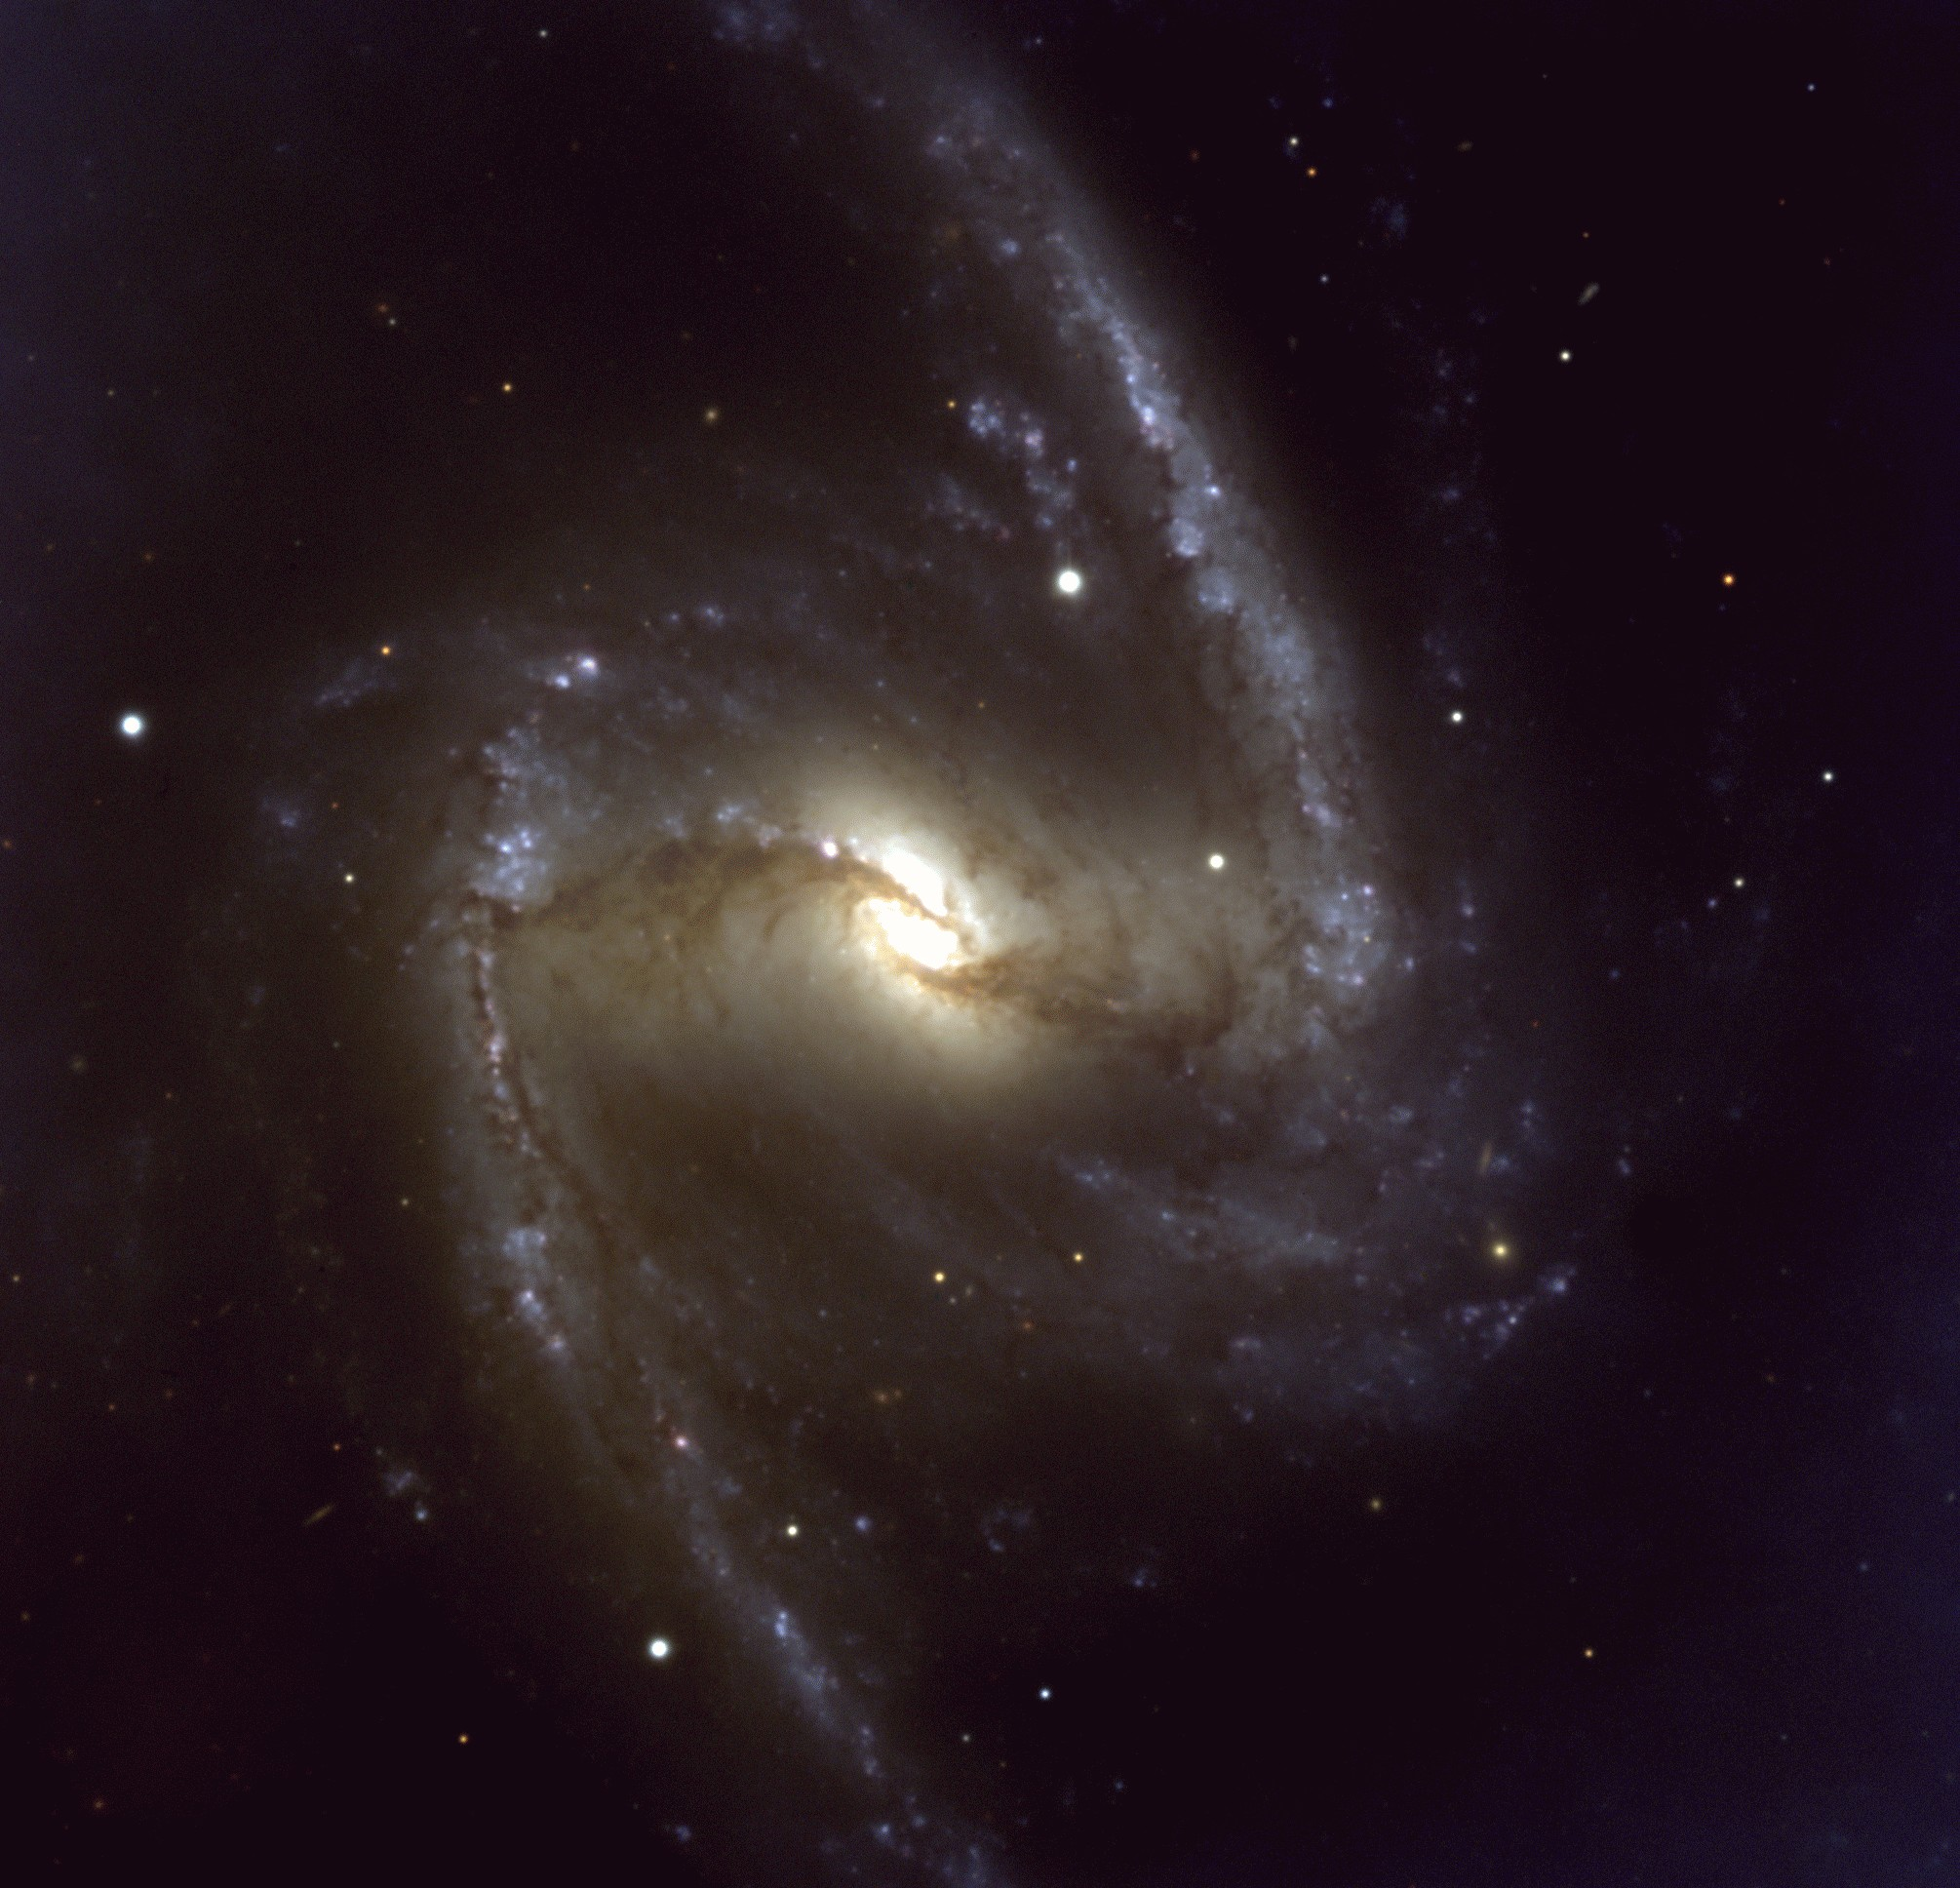
\includegraphics[width=4cm]{imagens/ngc_1365.jpg}} 
\qquad 
\subfigure[ref3][M109 (NGC 3992)]{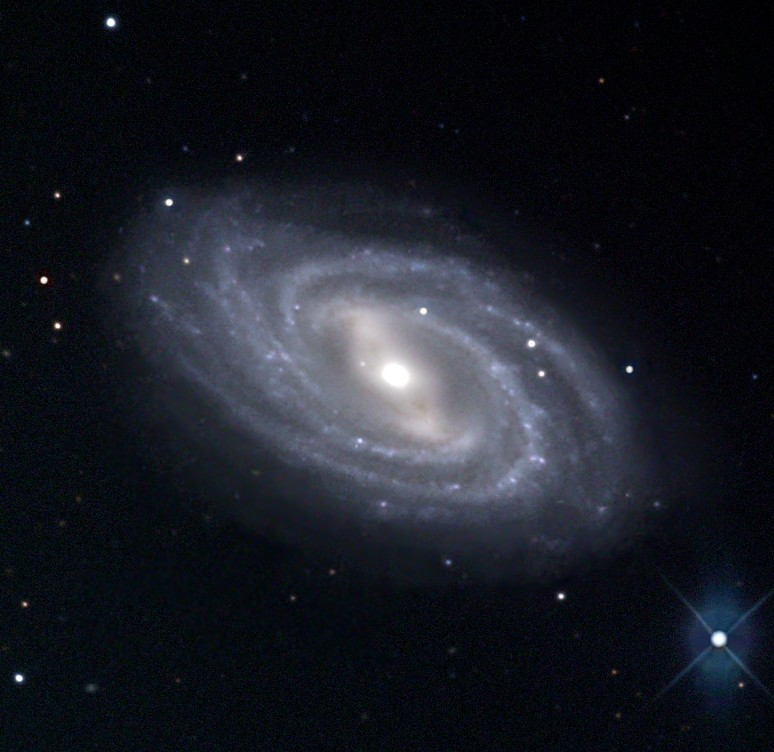
\includegraphics[width=4cm]{imagens/m109.jpg}} 
\caption{(a) NGC 1433. Galáxia do tipo SBa. A cerca de 32 milhões de anos-luz da Terra, é um tipo de galáxia muito ativa conhecida como galáxia Seifert - uma classificação que representa 10\% de todas as galáxias. Eles têm centros luminosos e muito brilhantes, comparáveis aos da nossa galáxia, a Via Láctea. Magnitude de 9.99. Crédito: ESA/Hubble. \newline (b) NGC 1365. Galáxia espiral-barrada do tipo SBb, a 60 milhões de anos-luz da Terra, na constelação da Fornalha. Magnitude de 9.5. É uma galáxia gigante com cerca de 200,000 anos-luz de diâmetro, ou seja, duas vezes o tamanho da Via Láctea. Crédito: FORS Team, VLT, ESO. \newline (c) M109 (NGC 3992). Galáxia espiral-barrada do tipo SBc, a 55 milhões de anos-luz da Terra, na constelação de Ursa Maior. Magnitude de 9.8. Crédito: Chris Lasley e Ray Galak} 
\label{fig:galáxias5} 
\end{figure} 

Nas espirais barradas, os braços normalmente partem das extremidades da barra. O fenômeno de formação da barra ainda não é bem compreendido, mas acredita-se que a barra seja a resposta do sistema a um tipo de perturbação gravitacional periódica (como uma galáxia companheira), ou simplesmente a consequência de uma assimetria na distribuição de massa no disco da galáxia \cite{bergh1998galaxy}. Alguns astrônomos também acreditam que a barra seja pelo menos em parte responsável pela formação da estrutura espiral, assim como por outros fenômenos evolutivos em galáxias. Nosso interesse não será classificar as galáxias com tamanha precisão, mas seria um trabalho relativamente possível com os métodos que serão aplicados. 

\subsection{Galáxias Irregulares} 

As galáxias irregulares são galáxias que apresentam uma estrutura morfológica desordenada, não possuem formas elípticas ou espirais \cite{bergh1998galaxy}. De modo que sua forma é indefinida. O tipo mais geral apresenta uma grande quantidade de estrelas recém-nascidas e uma produção de novas estrelas com uma certa intensidade. Hubble as classificou como galáxias irregulares devido à falta de qualquer simetria circular ou rotacional \cite{bergh1998galaxy}. Sua aparência sendo dominada por estrelas jovens brilhantes e nuvens de gás ionizado distribuídas irregularmente\cite{extragalatic}. Lembram as espirais no seu conteúdo estelar, que inclui estrelas de população jovens e velhas. 

As mais conhecidas são a Grande e a Pequena Nuvens de Magalhães, galáxias vizinhas da Via Láctea, visíveis a olho nu no Hemisfério Sul, foram identificadas pelo navegador português Fernão de Magalhães (1480-1521), em 1519.  

\begin{figure}[ht!] 
\centering 
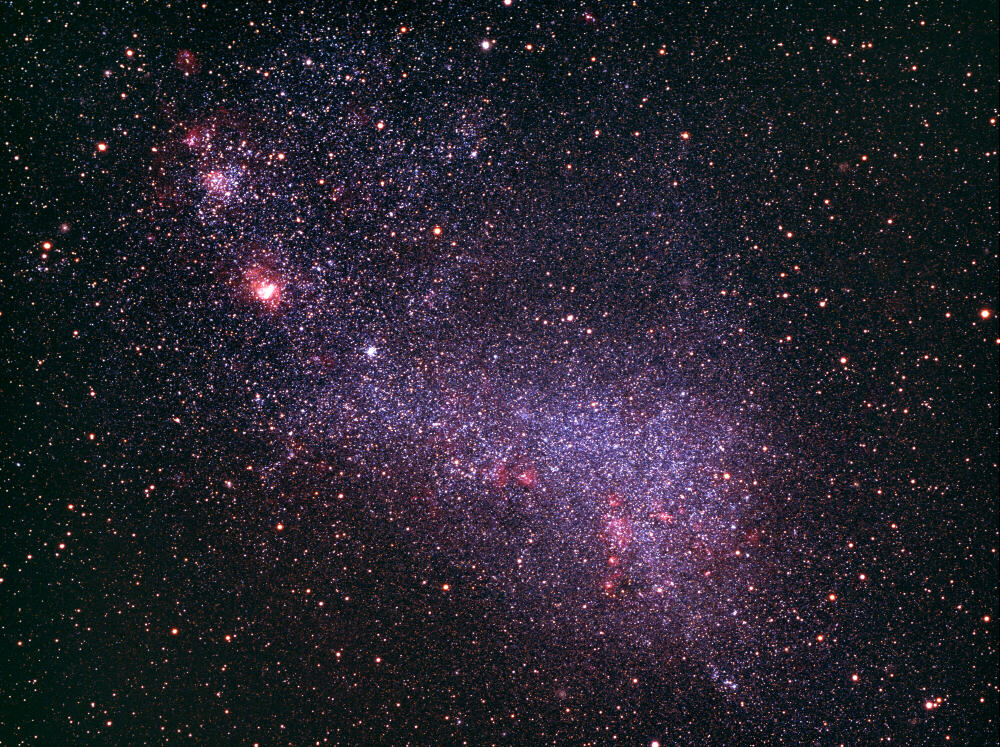
\includegraphics[width=12cm]{imagens/pequena_nuvem_magalhaes.jpg} 
\caption{A Pequena Nuvem de Magalhães é também conhecida como NGC 292. É uma galáxia anã irregular, em órbita da Via Láctea. Contém mais de 30 mil milhões de estrelas. A uma distância de 200 000 anos-luz, é uma das vizinhas mais próximas da nossa Galáxia. Situada na constelação do Tucano, é melhor visível no Hemisfério Sul. Forma um par com a Grande Nuvem de Magalhães Crédito: Observatório da Namíbia.}
\label{fig:PequenaNuvendeMagalhães} 
\end{figure} 

A Grande Nuvem de Magalhães orbita a Via Láctea, com velocidade de 387 km/s, o seu diâmetro é vinte vezes menor do que o da Via Láctea e o seu número de estrelas dez vezes menor. Sua morfologia é irregular, mas apresenta traços de uma estrutura espiralada. Sua constituição e compota de moléculas orgânicas complexas, como metanol, éter. 

Existe a especulação de que a Grande Nuvem de Magalhães já foi uma galáxia espiral barrada que rompeu da Via Láctea para tornar-se uma galáxia irregular. 

\section{Visão Computacional (VC)}\label{vc} 

O conceito de VC é muito amplo, mas geralmente se trata da extração de características presentes em imagens. Descrever características visuais possibilita compreendê-las computacionalmente e expande as possibilidades de aplicações possíveis. O objetivo básico é fornecer aos computadores recursos visuais semelhantes ao dos humanos de modo que as máquinas possam reconhecer determinado ambiente ou padrão. 

Dentro do AM utilizamos recursos de VC para as mais diversas aplicações, usando detectores de características visuais podemos coletar os padrões desejados para o aprendizado. A utilização de descritores de características tem como objetivo identificar um conjunto de pontos de interesse a partir do processo de varredura e identificação de pixels de interesse de determinada imagem, assim sendo cada método de detecção apresenta um algoritmo próprio, realizando a detecção de diferentes formas. 

Devido a isso, é possível analisar um determinado problema e suas particularidades, e consequentemente determinar quais algoritmos são mais indicados para a utilização \cite{Sonka1998}. Não existe uma regra geral para essa escolha devemos conhecer bem o conjunto de dados e testar. 

\subsection{Histogram of Oriented Gradients (HOG)} 

O HOG ou histograma de gradientes orientados é um descritor que usa o processamento de imagens para reconhecimento de padrões. A técnica conta ocorrências de orientação de gradientes em partes localizadas na imagem. 

A ideia geral por traz do HOG é que a aparência e a forma do objeto local dentro de uma imagem podem ser descritas pela distribuição de gradientes de intensidade ou direções das arestas. Dividindo a imagem em pequenas regiões conectadas chamadas células. E para cada célula um histograma de direções e criado. Assim pôr fim concatenamos estes histogramas para gerar o descritor. 

\subsection{Hu Moments (HM)} 

O HM ou momentos invariantes é um descritor que extrai contornos de um objeto em uma imagem, ao descrever a contorno de um objeto, podemos extrair um vetor de recurso de sua forma ou uma lista de números para representar a forma do objeto. Após extraído esta descrição podemos então comparar dois vetores de recurso usando uma métrica de similaridade ou uma função de distância para determinar quão "semelhantes" são as formas. 

Os momentos invariantes podem ser determinados por uma média ponderada das intensidades dos pixels da imagem, ou uma função desses momentos, geralmente escolhidos para ter alguma propriedade ou característica desejada, são úteis para descrever objetos após a uma segmentação. 

\section{Machine Learning (ML)}\label{ml} 

O termo machine learning ou aprendizado de máquina foi criado por volta 1959 pelo pioneiro da inteligência artificial, Arthur Samuel \cite{150082}, engenheiro do MIT, uma descrição básica naquela época era de um campo de estudo que dá aos computadores a habilidade de aprender sem terem sido programados para tal. 

O ML nos remete a ideia de máquinas e sistemas capazes de adquirir novos conhecimentos por conta própria, mas no geral ML são técnicas computacionais que nos permitem encontrar automaticamente padrões complexos e potencialmente úteis nos dados em geral, esses padrões são condensados em um modelo que pode ser usado em novos conjuntos de dados, um processo chamado de fazer predições ou realizar inferência. 

A operação básica desses algoritmos leva em conta uma construção de predição com análise dos dados ao invés de seguir instruções estáticas pré-programadas \cite{astroml}, diferente dos processos de inteligência artificial temos, aqui o aprendizado é essencialmente a fragmentação de um sistema para promover compreensão ou seja simplesmente procuramos padrões para promover comparações tendo em vista os dados, este aprendizado é o indutivo, o que significa que ele extrair regras e padrões de grandes conjuntos de dados. 

A construção de um modelo de AM é um processo desenvolvido em várias etapas, cada etapa apresenta os próprios desafios técnicos e conceituais \cite{astroml}. O tamanho dos conjuntos de dados de treinamento para modelos de AM reais pode alcançar ou ultrapassar facilmente a marca dos terabytes (TB).  

Por isso necessariamente precisamos de estruturas de processamento de dados em grande escala para esses conjuntos de dados de maneira eficiente e distribuída. Além disso, quando usamos um modelo de AM para fazer predições, é necessário aplicar as mesmas transformações usadas para os dados de treinamento nos novos conjuntos de dados, de modo que o conjunto de dados ativo seja apresentado ao modelo de AM da maneira esperada pelo modelo. 

\subsection{Modelos de Aprendizado de Máquina} 

Os modelos são especificações matemáticas ou probabilística aplicadas ao AM \cite{datascience}, e são essencialmente à criação e ao uso de modelos que aprendem a partir dos dados. Os modelos utilizados estão distribuídos nos seguintes grupos: métodos distância, métodos otimização, métodos probabilísticos e métodos de procura. Vamos trabalhar com alguns destes métodos, essencialmente a aplicação deles como técnicas de classificação que é o nosso interesse. 

\subsection{Naive Bayes (NB)} 

O classificador Naive Bayes é baseado no teorema de Bayes sendo um assim um classificador probabilístico simples \cite{datascience}. Chamado de método ingênuo de Bayes formando um conjunto de algoritmos de aprendizado supervisionado baseados na aplicação do teorema de Bayes com independência condicional entre cada par de recursos, dado o valor da variável de classe. 

O NB pode executar a classificação de um número arbitrário de variáveis independentes e geralmente é usado quando os dados têm muitos atributos. Os dados a serem classificados podem ser categóricos. Uma pequena quantidade de dados de treinamento é suficiente para estimar os parâmetros necessários.  

\subsection{Logistic Regression (LR)} 

A LR ou regressão logística é basicamente um modelo linear para classificação, também conhecida como regressão “logit”, classificação de entropia máxima ou classificador log-linear \cite{datascience}. A ideia deste modelo é que as probabilidades que descrevem os possíveis resultados são modeladas usando uma função logística, que podemos compreender como uma curva em formato de sigmoide regida pela equação de uma regressão logística.  

\subsection{Linear Discriminant Analysis (LDA)} 

O LDA ou analise de discriminante linear é uma generalização do discriminante linear de Fisher que é um método utilizado em estatística para encontrar combinações lineares de recursos que caracterizam ou separam classes, objetos ou eventos.  

A combinação resultante pode ser usada como um classificador linear ou para redução de dimensionalidade antes de uma classificação. Um classificador LDA tenta encontrar um limite linear que melhor separe as diferentes classes nos dados \cite{scikit-learn}.  

\subsection{K-Nearest Neighbors (K-NN)} 

O K-NN ou algoritmo dos K-vizinhos mais próximo é método baseado em distância. Dentre os algoritmos de ML o K-NN é o mais simples de todos \cite{datascience}. A intuição por trás do algoritmo é de que objetos próximos ou relacionados a um mesmo conceito são semelhantes entre si. 

O algoritmo do K-NN classifica um novo objeto com base nos exemplos do conjunto de treinamento que são próximos a ele. É um algoritmo  \textit(lazy), por não aprender um modelo compacto para os dados,  ele apenas memoriza os objetos já treinados. Uma das vantagens desse algoritmo é que ele pode ser utilizado tanto para problemas de classificação como para problemas de regressão de maneira direta.  

\subsection{Support Vector Machine (SVM)} 

As SVM ou máquina de vetores de suporte são um método de otimização, estas técnicas são eficazes para discriminar classes binária. A formulação básica é projetada para o problema de classificação linear, o algoritmo produz um hiperplano ideal, aquele que mantém a maior distância mínima de todos os dados de treinamento, sendo definida como a margem para separar entidades de diferentes classes. 

Por exemplo, se as duas classes pertencem a planetas habitáveis e não habitáveis, respectivamente, o problema é um problema de classificação binária e o hiperplano deve manter a maior distância possível dos pontos de dados de qualquer classe.  

\subsection{Decision Tree (DT)} 

O DT ou árvore de decisão é um método de procura onde existe uma construção logica de uma estrutura de dados em árvore que pode ser usada para classificação ou regressão. Cada um dos nós na árvore divide o conjunto de treinamento com base em um recurso, o primeiro nó é chamado nó raiz, que é baseado no recurso considerando o melhor preditor. Todos os outros nós da árvore são divididos em nós filhos com base em um certo critério de divisão ou regra de decisão que determina a fidelidade do objeto (dados) em particular à classe de recurso.  

Diz-se que um nó é mais puro se a probabilidade de classificar um determinado vetor de característica pertencente à classe $a_i$ em comparação com qualquer outra classe $a_j$, pois $i \not= j$ é maior \cite{scikit-learn}. Os nós devem ser nós puros, isto é, sempre que qualquer amostra de dados a ser classificada atingir um nó, ela deve ser classificada em uma das classes de dados com uma precisão muito alta.  

\subsection{Randon Forest (RF)} 

O RF ou floresta aleatória é um conjunto de várias árvores de decisão. Cada árvore é construída selecionando um subconjunto aleatório de atributos do conjunto de dados \cite{scikit-learn}. Cada árvore, por sua vez, realiza uma regressão ou uma classificação e uma decisão é tomada com base na previsão média (regressão) ou votação por maioria (classificação).  

A tarefa de classificar um novo objeto do conjunto de dados é realizada usando árvores construídas aleatoriamente.  Por exemplo, se uma floresta aleatória consiste em dez árvores de decisão, das quais seis classificam um vetor de característica como pertencente à uma classe \textit{a}  e as quatro árvores restantes classificam outra classe \textit{b}, então podemos concluir que o RF classificou o vetor como sendo da classe \textit{a}.  

\subsection{Multilayer Perceptron (MLP)} 

Um MLP ou perceptron multicamada é uma classe de rede neural artificial. O termo MLP é uma rede composta por múltiplas camadas. As multicamadas perceptrons são algumas vezes chamadas como redes neurais. Um MLP básico consiste em pelo menos três camadas de nós: uma camada de entrada, uma camada oculta e uma camada de saída. Após os nós de entrada, cada nó é um neurônio que usa uma função de ativação não linear. O MLP utiliza uma técnica de aprendizado supervisionado chamada "backpropagation" para o treinamento \cite{astroml}.  

A nossa utilização do MLP se restringira a classificação, onde implementamos um algoritmo perceptron de várias camadas que treina usando a retro propagação, basicamente treinamos duas matrizes, que mantém as amostras de treinamento representadas como vetores de recurso e matriz de tamanho, que mantém os valores de destino (rótulos de classe) para as amostras de treinamento.  

Após o treinamento, o modelo pode prever rótulos para novas amostras, ajustando um modelo não linear aos dados de treinamento que contém as matrizes de peso que constituem os parâmetros do modelo. Destas matrizes podemos criar o modelo capaz de discernir se um novo objeto (matriz) e de uma determinada classe ou de outra classe. 

	% Metodologia
	\chapter{Metodologia} 

O nosso trabalho consiste em criar um modelo de AM capaz de classificar ou rotular uma imagem em sua respectiva classe com a ajuda de recursos aprendidos de centenas de imagens, para isso devemos seguir passos básicos a todos modelos de AM como: a coleta de dados, a preparação dos dados, a escolha do modelo, o treinamento, a avaliação do modelo e por fim testar o quão preditivo é o nosso modelo.  

Neste capítulo vamos trazer os passos seguidos na construção do modelo de AM que serão empregados para ambos os conjuntos de dados que serão utilizados Galaxy Zoo (GZ) e DSS-RC3 , desde a coleta de dados até uma análise dos modelos e uma comparação entre os mesmo, e por fim vamos usar o modelo que melhor desempenhou e fazer uma análise estatística da predição deste modelo. Inicialmente vamos descrever os passos seguido na construção do processo de aprendizado e ao final vamos aplicar esses passos nos nossos conjuntos de dados. 

Podemos ressalvar que são dois processos distintos o aplicado ao GZ é mais simples e aconteceu em um momento posterior ao início  da pesquisa onde já havia um certo conhecimento da montagem de um dataset \footnote{Vamos introduzir a ideia de "dataset", de forma simples se trata de uma coleção de dados normalmente tabulado, onde cada elemento (ou indivíduo) tem várias características. Cada coluna representa uma variável particular. Cada linha corresponde a um determinado membro do conjunto de dados em questão. Cada valor é conhecido como um dado. O conjunto de dados pode incluir dados para um ou mais membros, correspondente ao número de linhas.} e das técnicas de AM. O processo dos dados do DSS-RC3 pode ser classificado como o real processo de montagem de um conjunto de dados para aplicação de técnicas de AM, ele não foi linear, em diversos momentos, tivemos que fazer uma nova coleta das imagens com parâmetros diferentes, o treino deste dataset aconteceu bem depois de termos o montado inicialmente a ideia era utilizar de técnicas de aprendizado profundo, mas optamos pelo AM por ser mais simples e por apresentar um aprendizado mais profundo do assunto aqui tratado. 

\section{Coleta de dados} 

Em 1609 todas as observações astronômicas eram feitas a olho nu, foi nesse ano que Galileu Galilei, tendo ouvido falar sobre um instrumento capaz de aproximar as imagens, construiu uma luneta, e pela primeira vez, o homem pode ver o céu de mais perto e assim a observação evoluiu até onde estamos no presente momento, o cenário não e mais tão simples hoje temos a nossa mão uma infinidade de observações e que geram dados na casa dos TB, e grande parte deste dados estão disponíveis abertamente para qualquer pessoa com acesso à internet.  

A facilidade de coleta muitas vezes é um problema pois se torna difícil escolher um bom conjunto de dados, em ML é de extrema importância esta coleta com foco no que se necessita para executar um bom aprendizado. Nosso objetivo foi procurar um conjunto de dados oficiais de imagens de galáxias que possibilitasse uma classificação morfológica.  

É importante dizer que teremos duas abordagens nesse item uma que irá tratar dos dados do GZ que já estão separados e que nos resta explicar a separação e dizer como foram utilizadas as imagens, a segunda abordagem será para os dados do RC3, que demandou um processo típico de montagem de um dataset, desde o processo de coletar até a parte de amostragem da imagens. 

\section{Preparação dos dados} 

A preparação de dados para treinamento do modelo de AM leva em conta diversas metodologias desde separações simples até modelos estatísticas de amostragem, o modelo mais simples leva em conta a divisão disponibilizada pelo próprio conjunto de dados. Com esses dados já divididos temos que extrair os recursos, que são as informações ou lista de números extraídos de uma imagem. Existem diversos algoritmos de extração de recursos vamos usar aqueles que descrevemos na seção \ref{vc}. 

\subsection{Extração de recursos}

Quando decidimos as características que podemos usar para quantificar imagens de galáxias, podemos pensar, em forma e luminosidade como as principais. Esta é uma escolha óbvia para quantificar globalmente e representar a imagem de uma galáxia. Mas quando desejamos classifica-las encontramos uma certa dificuldade, o grande problema é que mesmo para um profissional treinado algumas galáxias apresentam uma classificação dúbia.  

Uma abordagem que pode produzir bons resultados, é a escolha de vários atributos descritivos de característica, já que algumas galáxias apresentam muito em comum. Portanto, precisamos quantificar a imagem combinando diferentes descritores de recursos para que ela descreva a imagem de forma mais eficaz. 

\subsection{Concatenação do descritor global}

Existem duas classes de descritores os globais e os locais \cite{Sonka1998}. Os globais são descritores de recursos que quantificam uma imagem globalmente. Eles não possuem o conceito de pontos de interesse e, portanto, levam toda a imagem para processamento. Os descritores locais quantificam as regiões locais de uma imagem, os pontos de interesse são determinados em toda a imagem e os fragmentos da imagem ao redor desses pontos de interesse são considerados para análise. 

Os vetores de recursos globais, podem ser apenas concatenados de formas simples onde cada vetor de recurso formar um único vetor que finalmente e concatenado em único descritor global. Vamos usar essa abordagem, para os vetores de recursos locais, bem como combinações de vetores de recursos globais e locais, iriamos precisar de algo chamado Bag of Visual Words (BOVW), que foi estudado, mas percebemos ser inviável para o nosso caso por isso não será implementado. 

\section{Escolha do modelo} 

 Os modelos escolhidos foram os citados na seção (\ref{ml}), agora necessitamos analisar o desempenho da classificação de cada modelo e procurar entender a diferença geral da qualidade no aprendizado esse é um aspecto muito importante para que tenhamos um modelo de AM realmente capaz de executar nossa tarefa de predição. Como já temos um descritor global criado no passo anterior podemos apenas utiliza-lo para treinar rapidamente os modelos e fazer análise comparativa inicial. 

 Para este passo precisamos criar nossos modelos de AM neste ponto contamos com o Scikit-learn (SL). O SL é uma biblioteca de aprendizado de máquina de código aberto que oferece suporte ao aprendizado supervisionado e não supervisionado \cite{scikit-learn}. Ele também fornece várias ferramentas para ajuste de modelo, pré-processamento de dados, seleção e avaliação de modelo e muitos outros utilitários, grande parte do estudo aqui apresentado vai utilizar da biblioteca SL. 

Uma observação importante é que todos os modelos escolhidos se apresentam implementados na biblioteca do SL. Uma breve descrição sobre os mesmos foi feita na introdução. Para entender melhor esses algoritmos vide a fonte didática utilizada \footnote{\citeonline{astroml}, \citeonline{astroml2} e \citeonline{datascience}}. Usaremos também a funções fornecida pela SL para dividir nosso conjunto de dados de treinamento dados de treino e dados de teste. Desta forma, treinamos os modelos com dados de treino e testamos o modelo treinado com os dados de teste, ou seja, dados não visto anteriormente. O tamanho da divisão é decidido pelo parâmetro que devemos definir, essa divisão leva em conta muito do queremos para nosso modelo e da disponibilidade inicial do conjunto de dados. 

\section{Treinamento} 

 O treinamento acontece após toda a montagem do nosso dataset onde já extraímos, concatenamos e salvamos recursos globais e rótulos de nosso conjunto de dados de treinamento. Precisamos agora criar nossos modelos de AM, nestes pontos contamos com a ajuda do SL os modelos escolhidos estão na seção (\ref{ml}). O entendimento completo destes algoritmos ficaria fora do escopo deste trabalho visto que poderíamos desenvolver um projeto de pesquisa sobre apenas um modelo. A ideia por traz de trazer vários modelos é procurar aprender como os mesmo e ver aquele que apresenta um melhor desempenho com o nosso tipo de dado. 

Utilizamos também do SL para dividir nosso conjunto de dados de treinamento em dois tipos de conjuntos, teste e treino. Assim, treinamos os modelos com treino e testamos o modelo treinado com teste que não foi visto anteriormente. O tamanho da divisão é decidido por um parâmetro previamente escolhido, na literatura \cite{astroml2} vemos em diversos momento uma divisão de 80\% para treino e 20\% teste a empregada aqui será está. 

\subsection{Analise de comparação entre os modelos}

Aplicamos também técnicas de K-Fold Cross Validation, que são utilizadas na validação de modelos. Em resumo, se escolhermos K = 10, dividimos todos os dados em 9 partes para treinamento e uma parte para teste exclusivamente em cada rodada, este processo acontece em cada época de treino até o mesmo ser completado. Para entender mais sobre isso, recomendo uma leitura rápida no artigo \citeonline{VanwinckelenGitte2012Oema}. 

Após importar todos os modelos do SL treinamos com nossos recursos armazenados. O dataset está salvo localmente e apresenta um formato de arquivo .h5 que é um conjunto de formatos de arquivos e bibliotecas criadas para organização e armazenamento de grandes quantidades de dados numéricos, é uma boa opção pois podemos utilizar esse mesmo dataset em outros projetos. O tempo treino leva em conta diversos parâmetros desde os mais lógicos como o tamanho do dataset até ajustes mais refinados \cite{astroml}. 

\section{Avaliação} 

O passo mais importante de um modelo de AM é a construção do dataset e em segundo lugar podemos colocar a avaliação, neste aspecto é um momento decisivo para saber se o nosso modelo apresentou desempenho desejado, neste ponto e onde temos que decidir mexer nos passos anteriores ou não, para isso treinamos cada um dos modelos de AM que escolhemos e verificamos os resultados da validação cruzada (K-Folds), os dados utilizados para essa comparação serão apenas os dados de treino. 

Após a avaliação inicial de todos os modelos precisamos escolher aquele que apresentou o melhor desempenho e aplicar outros testes para verificar sua eficiência. Podemos fazer alguns comentários sobre o que esperamos das técnicas e sobre suas precisões, mas o aspecto mais importante neste ponto e o tamanho da amostra que mostra que nem sempre uma amostra maior vai apresentar melhores resultados. Precisamos de grandes quantidades de dados para obter melhor precisão, mas devemos notar a qualidade desses dados e a precisão dos mesmos. 

Um ponto importante nos testes de AM é o teste de pequenos conjuntos de dados, isso nos dá uma ideia geral de correções pequenas ou grandes que devemos executar no nossos dados ou processos de treino, também evita o excesso no tempo de execução de treinamento, algo desejável quando temos uma grande amostra que facilmente pode levar horas ou dias pra executar um ciclo de treino, ao longo deste trabalho não tivemos que utilizar uma máquina com potencial computacional muito alta mas alguns treinos levaram horas. 

\section{Aprimoramento dos parâmetros}

O aprimoramento de parâmetros visa melhorar a qualidade e a eficiência do modelo de AM, essa etapa é importante para identificar valores que afetam diretamente a acurácia do modelo e o tempo de treinamento necessário. Os principais parâmetros a serem analisados aqui é o quanto a linha de AM é alterada de acordo com a informação adquirida no procedimento anterior, testamos novas possibilidades para analisar melhor os modelos treinados e ensaiar formas de como aprimorar os mesmos. 

É importante destacar que, antes de começar a frase, deve-se estabelecer quais serão as definições de um bom modelo, pois elas guiarão o aprimoramento dele. Afinal, os ajustes e melhorias que serão feitos dependem da base de dados, do modelo e do treinamento. Considerando tudo isso, o processo de AM deve ser continuado apenas quando o aprimoramento dos parâmetros for alcançado. Neste ponto iremos testa aumentar o numero de itens da amostra e treinar descritores novos ou separados buscando aperfeiçoar nossos modelos e adquirir uma acurácia melhor.

\section{Predição}

Como nossa tarefa inicial era classificação, desejamos ao final mesma utilizar os modelos treinados com essa base para predizer a classificação de um galaxia. O objetivo é encontrar uma função a partir dos dados de treinamento que possa classificar um objeto novo e desconhecido na classes que treinamos ou seja desejamos rotular ou dar uma “classe” a um padrão. Na predição ou classificação, baseado em dados de imagens de galaxias, um novo padrão poderia ser classificado em duas possíveis classes, “espital” ou “elíptica”. Também se diz que os métodos de AM dessa natureza seguem o paradigma supervisionado, pois é necessário apresentar ao método uma série de dados já rotulados para que o método possa aprender.


	
	% Projetos
	\chapter{Galaxy Zoo} 

O GZ é um projeto de astronomia "on-line" onde somos convidados a classificar galáxias, a ideia inicial usar a mão de obra do público em geral na pesquisa científica \cite{Raddick_2010}. Sendo hospedado em um site onde qualquer pessoa com conexão à Internet é convidada a participar da pesquisa classificando galáxias do SDSS. O projeto fez tanto sucesso que em abril de 2009, mais de 200 000 voluntários haviam feito mais de 100 milhões de classificações de galáxias. 

Podemos facilmente encontrar estes dados prontos e com uma certa facilidade no Kaggle, que é empresa subsidiária da Google LLC, é conta com uma comunidade on-line de cientistas de dados e profissionais de AM. O Kaggle permite que os usuários encontrem e publiquem conjuntos de dados, explorem e construam modelos em um ambiente de ciência de dados baseado na web, existem diversos desafios que são colocados pelo Kaggle e nosso conjunto de dados do GZ se trata de um desses conjuntos usados em um desafio. 

\begin{figure}[!ht] 
\centering 
\subfigure[ref1][Galaxias Espirais]{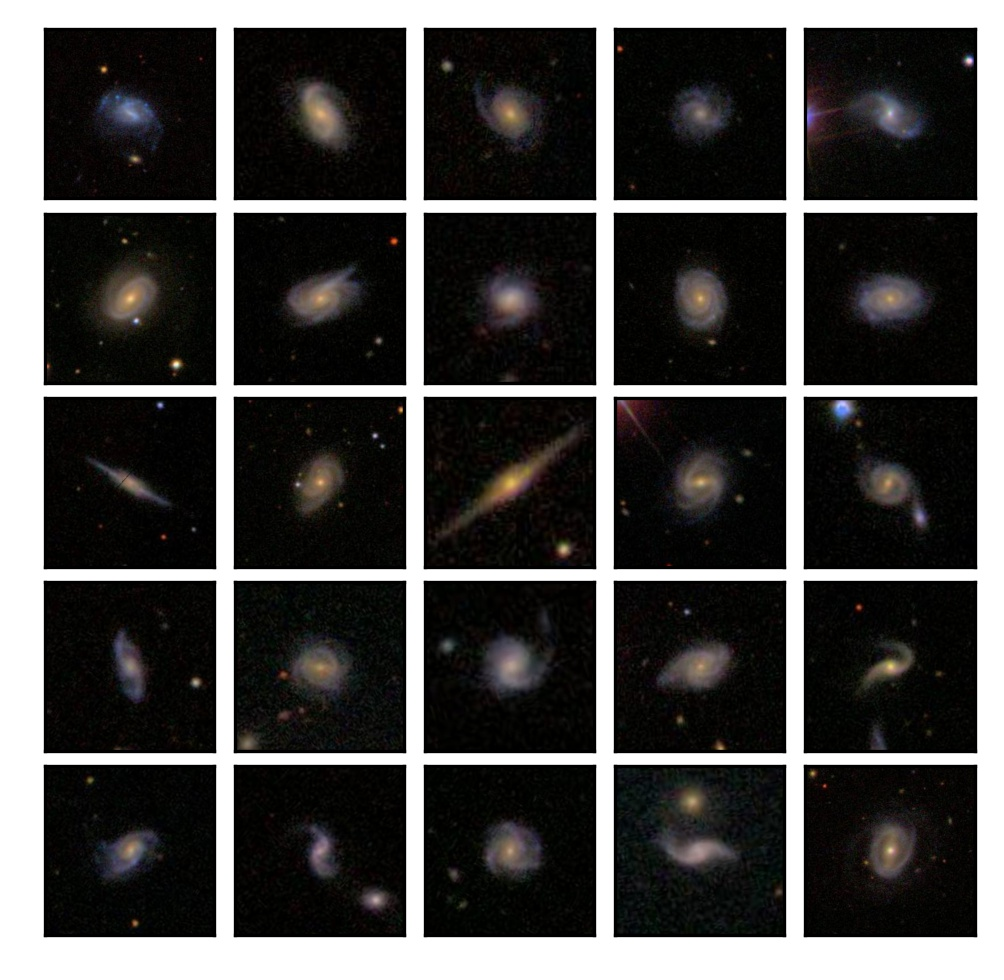
\includegraphics[width=6cm]{imagens/teste1.jpg}} 
\qquad 
\subfigure[ref2][Galaxias Elípticas]{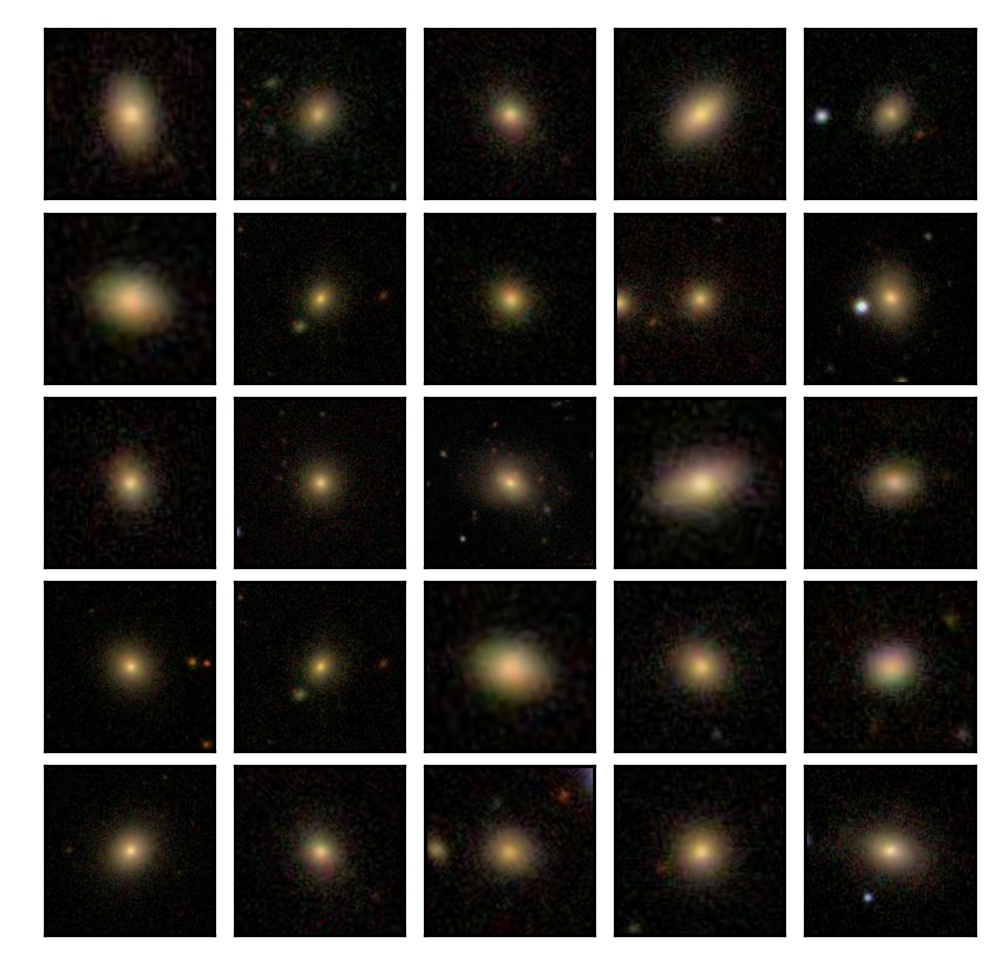
\includegraphics[width=6cm]{imagens/teste2.jpg}} 
\caption{(a) Amostra aleatória de galáxias classificadas como espirais no conjunto de dados do GZ. (b) Amostra aleatória de galáxias classificadas como elípticas no conjunto de dados do GZ.} 
\label{fig:juwdidj} 
\end{figure} 
\subsection{Descrição dos dados} 

Os dados consistem exclusivamente em imagens as quais já foram classificadas seguindo as perguntas feitas no site do GZ, temos um arquivo no formato de planilha que nos traz as informações vinculadas das imagens.  

A primeira coluna é identidades das imagens como GalaxyID, este é um ID gerado aleatoriamente que permite apenas que você combine as distribuições de probabilidade com as imagens. As próximas 37 colunas são todos números de ponto flutuante entre 0 e 1 inclusive. Estes representam a morfologia (ou forma) da galáxia em 37 categorias diferentes, conforme identificado por classificações de voluntários crowdsourced como parte do projeto GZ 2.  

Essas morfologias estão relacionadas às probabilidades de cada categoria, um número alto (próximo a 1) indica que muitos usuários identificaram esta categoria morfológica como sendo de uma galáxia com um alto nível de confiança. Números baixos para uma categoria (perto de 0) indicam que o recurso provavelmente não está presente. 

 
	\chapter{Third Reference Catalog of Bright Galaxies} 

	
	% Conclusão
	\chapter{Considerações Finais}
% Nada de mais por aqui.

\section{Um breve historia do caminho até aqui}

\subsection{Modelos usados}

\section{Analise do processo de predição}

	% Elementos pós-textuais
	\postextual
	% Os elementos a seguir aparecerão ao final do artigo.

% Referências bibliográficas
\bibliography{refs}

% Glossário
% Consulte o manual da classe abntex2 para orientações sobre o glossário.
%\glossary

% Apêndices
\begin{apendicesenv}
% Imprime uma página indicando o início dos apêndices
\partapendices
%
\chapter{1}
%nada aqui

\chapter{2}
%nada aqui

\end{apendicesenv}

% Anexos
\begin{anexosenv}
% Imprime uma página indicando o início dos anexos
\partanexos

\chapter{1}
%nada aqui


\chapter{2}
%nada aqui

\end{anexosenv}


% INDICE REMISSIVO
\phantompart
\printindex
	
	% Referências bibliográficas
	\bibliography{refs}


\end{document}
